\chapter{External Specification}

This chapter provides a detailed overview of the external specifications for the application. It outlines the specific requirements for its operation and the installation procedures necessary for a straightforward setup. Additionally, it includes key information to improve user understanding and ensure the application fulfils its intended purpose effectively.

\section{Hardware and Software Requirements}
\subsection{Hardware Requirements}
\begin{itemize}
    \item Android smartphone with Android 11.0 (API level 30) or higher.
    \item Camera with support for CameraX.
     \item Minimum 2GB RAM for standard use of the application, or 3GB RAM for optimal performance on devices with lower memory and processing power.
    \item Internet connection for the dice recognition module; the other parts of the app do not require internet and will work otherwise.
    \item At least 100MB of free storage space.
    \item Processor: ARM-based processor supporting Neon instruction set.
\end{itemize}

\subsection{Software Requirements}
To build the application, the following software is required:
\begin{itemize}
    \item Android Studio Giraffe (2023.1.1) or later.
    \item Kotlin 2.0.21
    \item Gradle 8.10.2 and the corresponding Android Gradle Plugin (e.g. 8.1.2).
    \item CameraX library version: 1.4.0.
\end{itemize}

\section{Installation Procedure}
For installing the application, the following procedure is required:

\subsection{APK Download}
\begin{enumerate}
    \item Download the Release APK from the project's repository at \href{https://github.com/Mayokun-Sofowora/kavi/releases/download/v1.0.0/app-release.apk}{GitHub Releases Page}.
    \item Enable installation from unknown sources in the device's settings. Note that installing apps from unknown sources has security implications; please proceed with caution.
    \item Open the APK file and follow the on-screen instructions.
\end{enumerate}

\subsection{Building with Android Studio}
To install the application for debugging purposes, follow these procedures:
\begin{enumerate}
    \item \textbf{Clone the Repository}: Start by cloning the project repository from GitHub.
    \begin{verbatim}
        git clone https://github.com/Mayokun-Sofowora/kavi.git
    \end{verbatim}
    \item \textbf{Open in Android Studio}: Launch Android Studio and open the cloned project.
    \item \textbf{Sync Gradle Dependencies}: Allow Android Studio to sync the Gradle dependencies automatically.
    \item \textbf{Run on Device/Emulator}: Connect an Android device or start an emulator with a minimum SDK of 30, then run the application.
\end{enumerate}

In addition to the instructions provided, be sure that:
\begin{itemize}
    \item  A debug build variant is selected in Android Studio.
    \item USB debugging is enabled in the device's settings.
    \item You connect an Android device via USB or use an emulator.
    \item  You select the appropriate run configuration in Android Studio.
\end{itemize}

\section{Types of Users}
\begin{itemize}
    \item \textbf{Regular Users}: Play dice games, use image recognition features, and adjust settings.
    \item \textbf{Developers/Testers}: Access debugging logs, experimental features, and perform system administration tasks.
\end{itemize}

\section{User Manual}
\label{sec:user_manual}

\subsection{Navigating the App}

When starting the game, users are welcomed with a splash screen that displays the application's logo in figure~\ref{fig:splash_screen}. After a short moment, the main menu is shown in figure~\ref{fig:main_menu}. The main menu provides navigation options to access the different features of the application.
\begin{figure}[h]
    \centering
    \begin{subfigure}[b]{0.27\textwidth}
        \centering
        \fbox{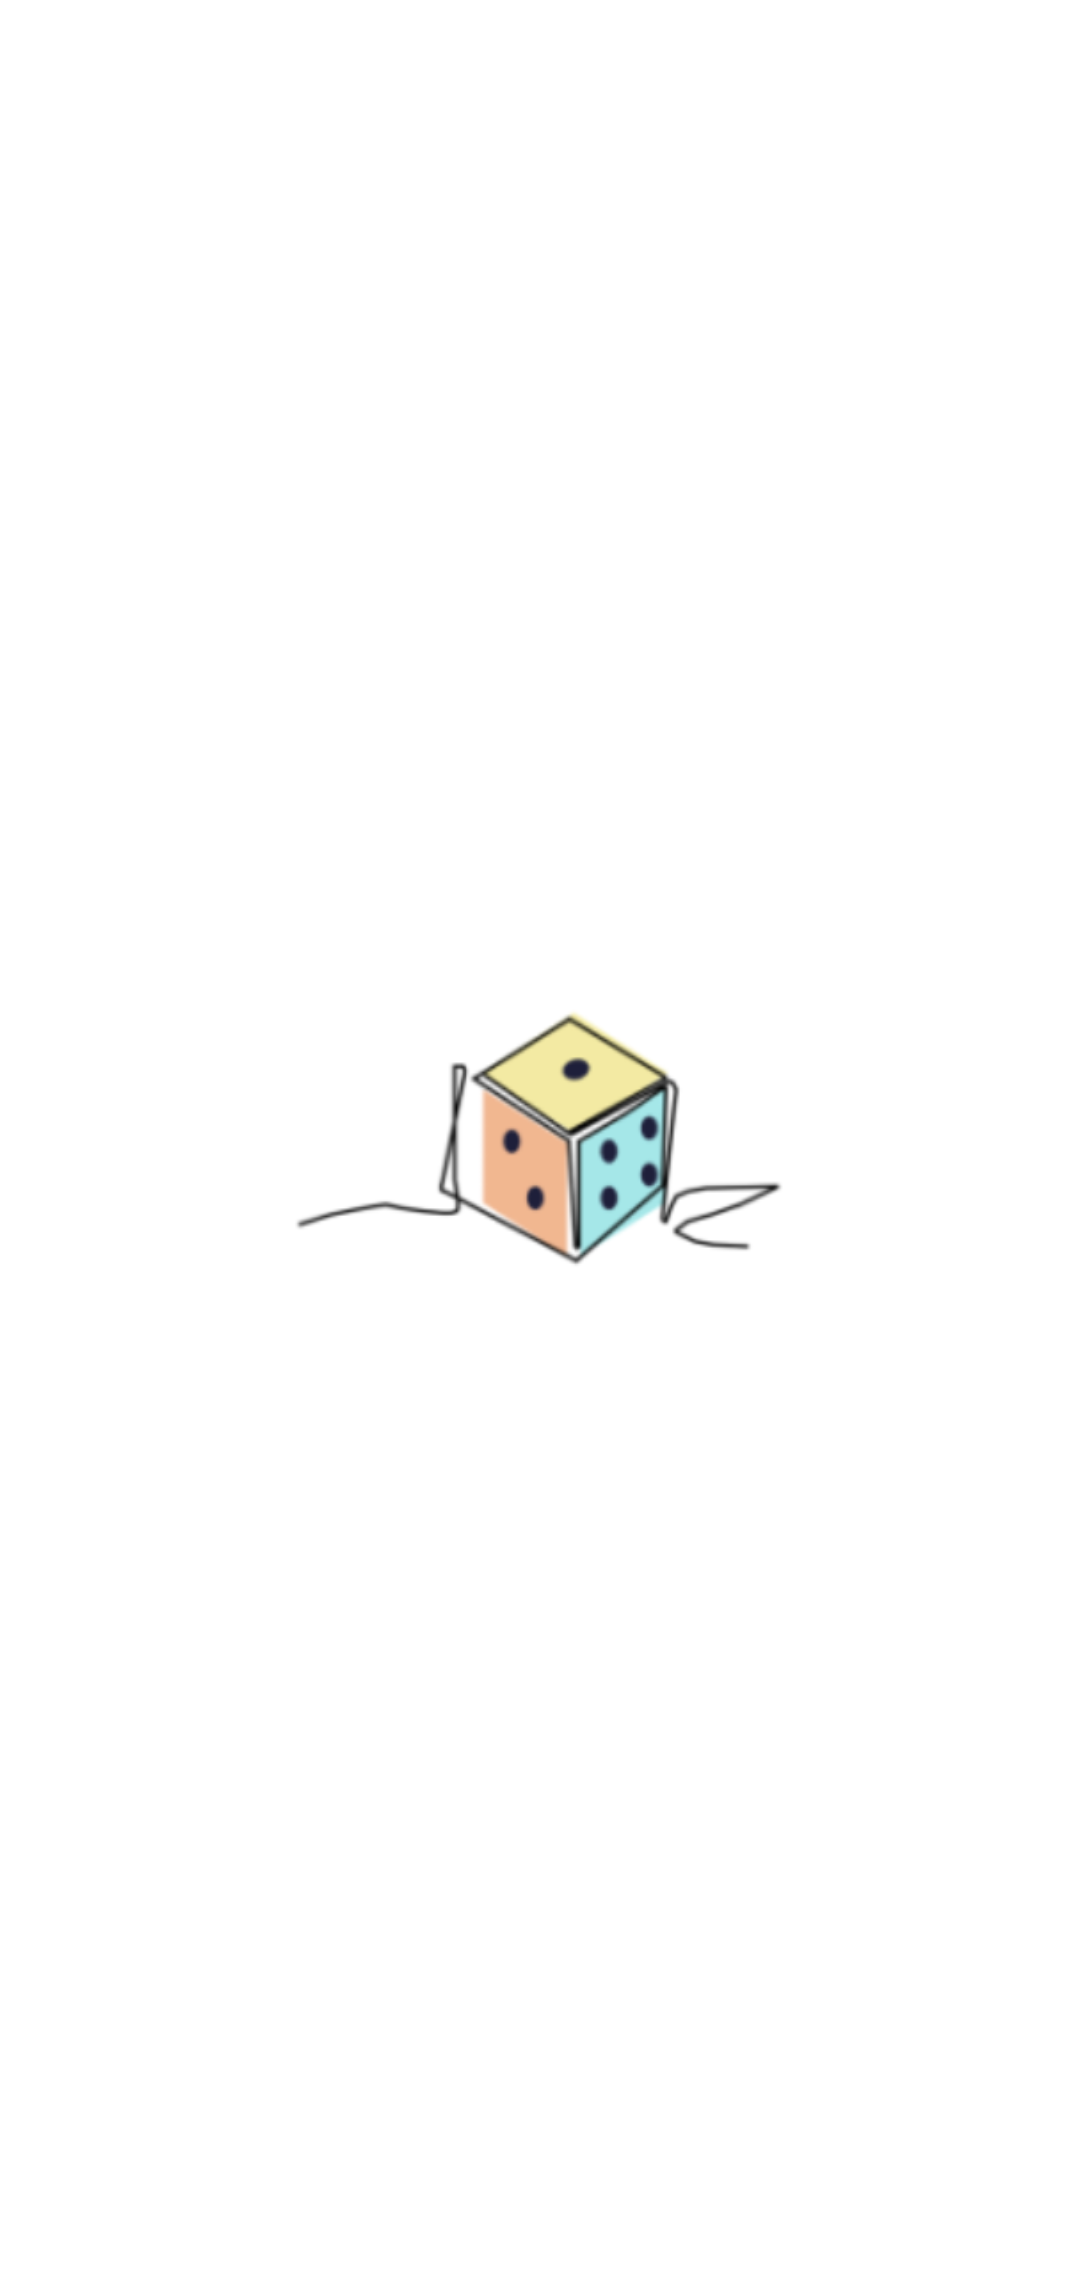
\includegraphics[width=\textwidth]{img/splash screen.png}}
        \caption{The Splash Screen}
        \label{fig:splash_screen}
    \end{subfigure}
    \hspace{1em}
    \begin{subfigure}[b]{0.27\textwidth}
        \centering
        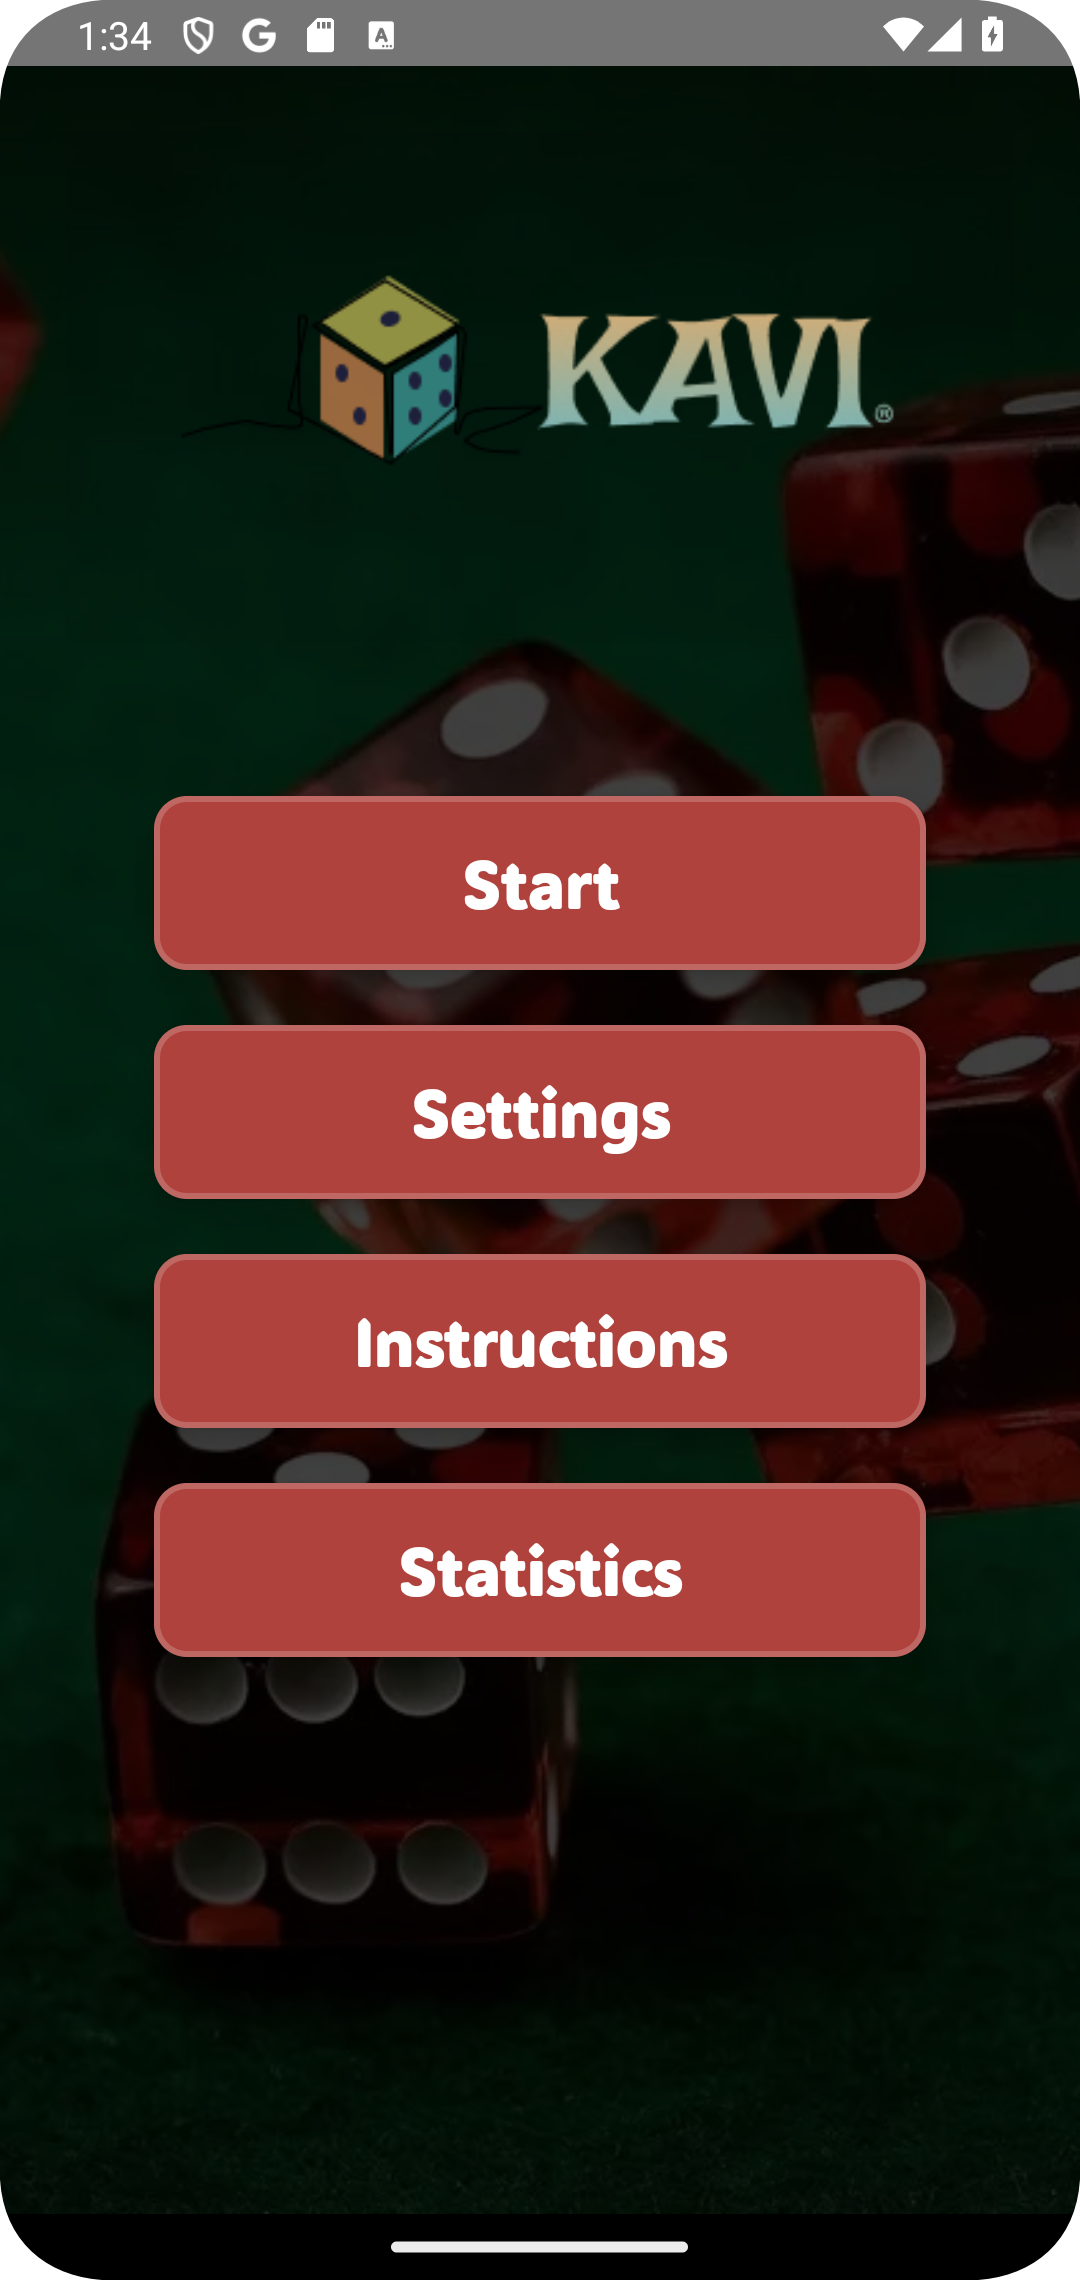
\includegraphics[width=\textwidth]{img/main menu.png}
        \caption{The Main Menu}
        \label{fig:main_menu}
    \end{subfigure}
    \caption{Screens displayed when starting the game.}
    \label{fig:starting_game}
\end{figure}

\subsection{Game Interface}

The interface allows users to navigate to different sections of the application, such as the classic boards to play the classic dice games or the virtual screen to use the image recognition feature. The figure~\ref{fig:interface_mode} shows the navigation options available.

\begin{figure}[h]
    \centering
    \begin{subfigure}[b]{0.27\textwidth}
        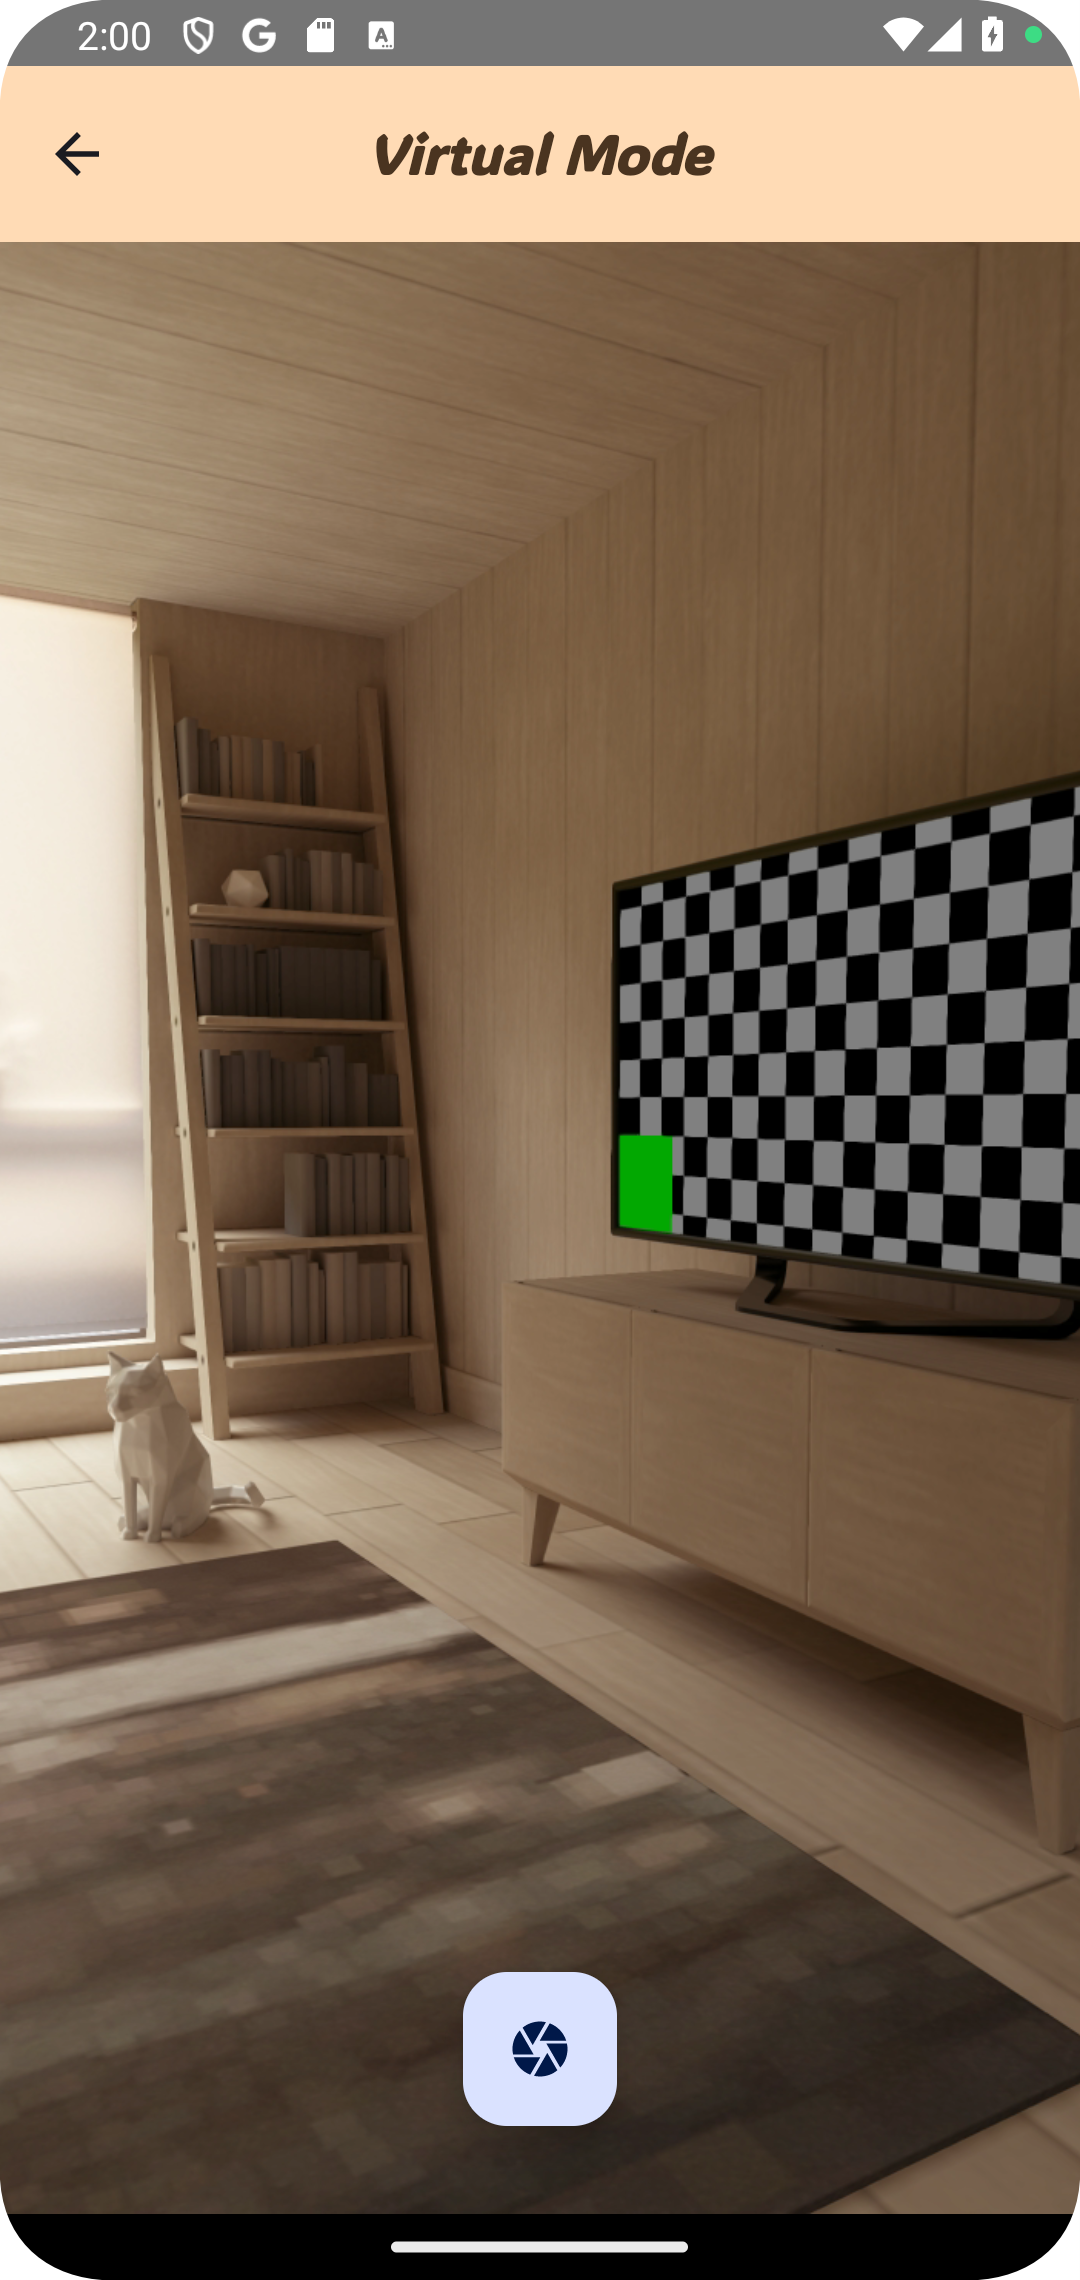
\includegraphics[width=\textwidth]{img/virtual mode.png}
        \caption{Virtual Mode}
        \label{fig:virtual_mode}
    \end{subfigure}
    \hfill
    \begin{subfigure}[b]{0.27\textwidth}
        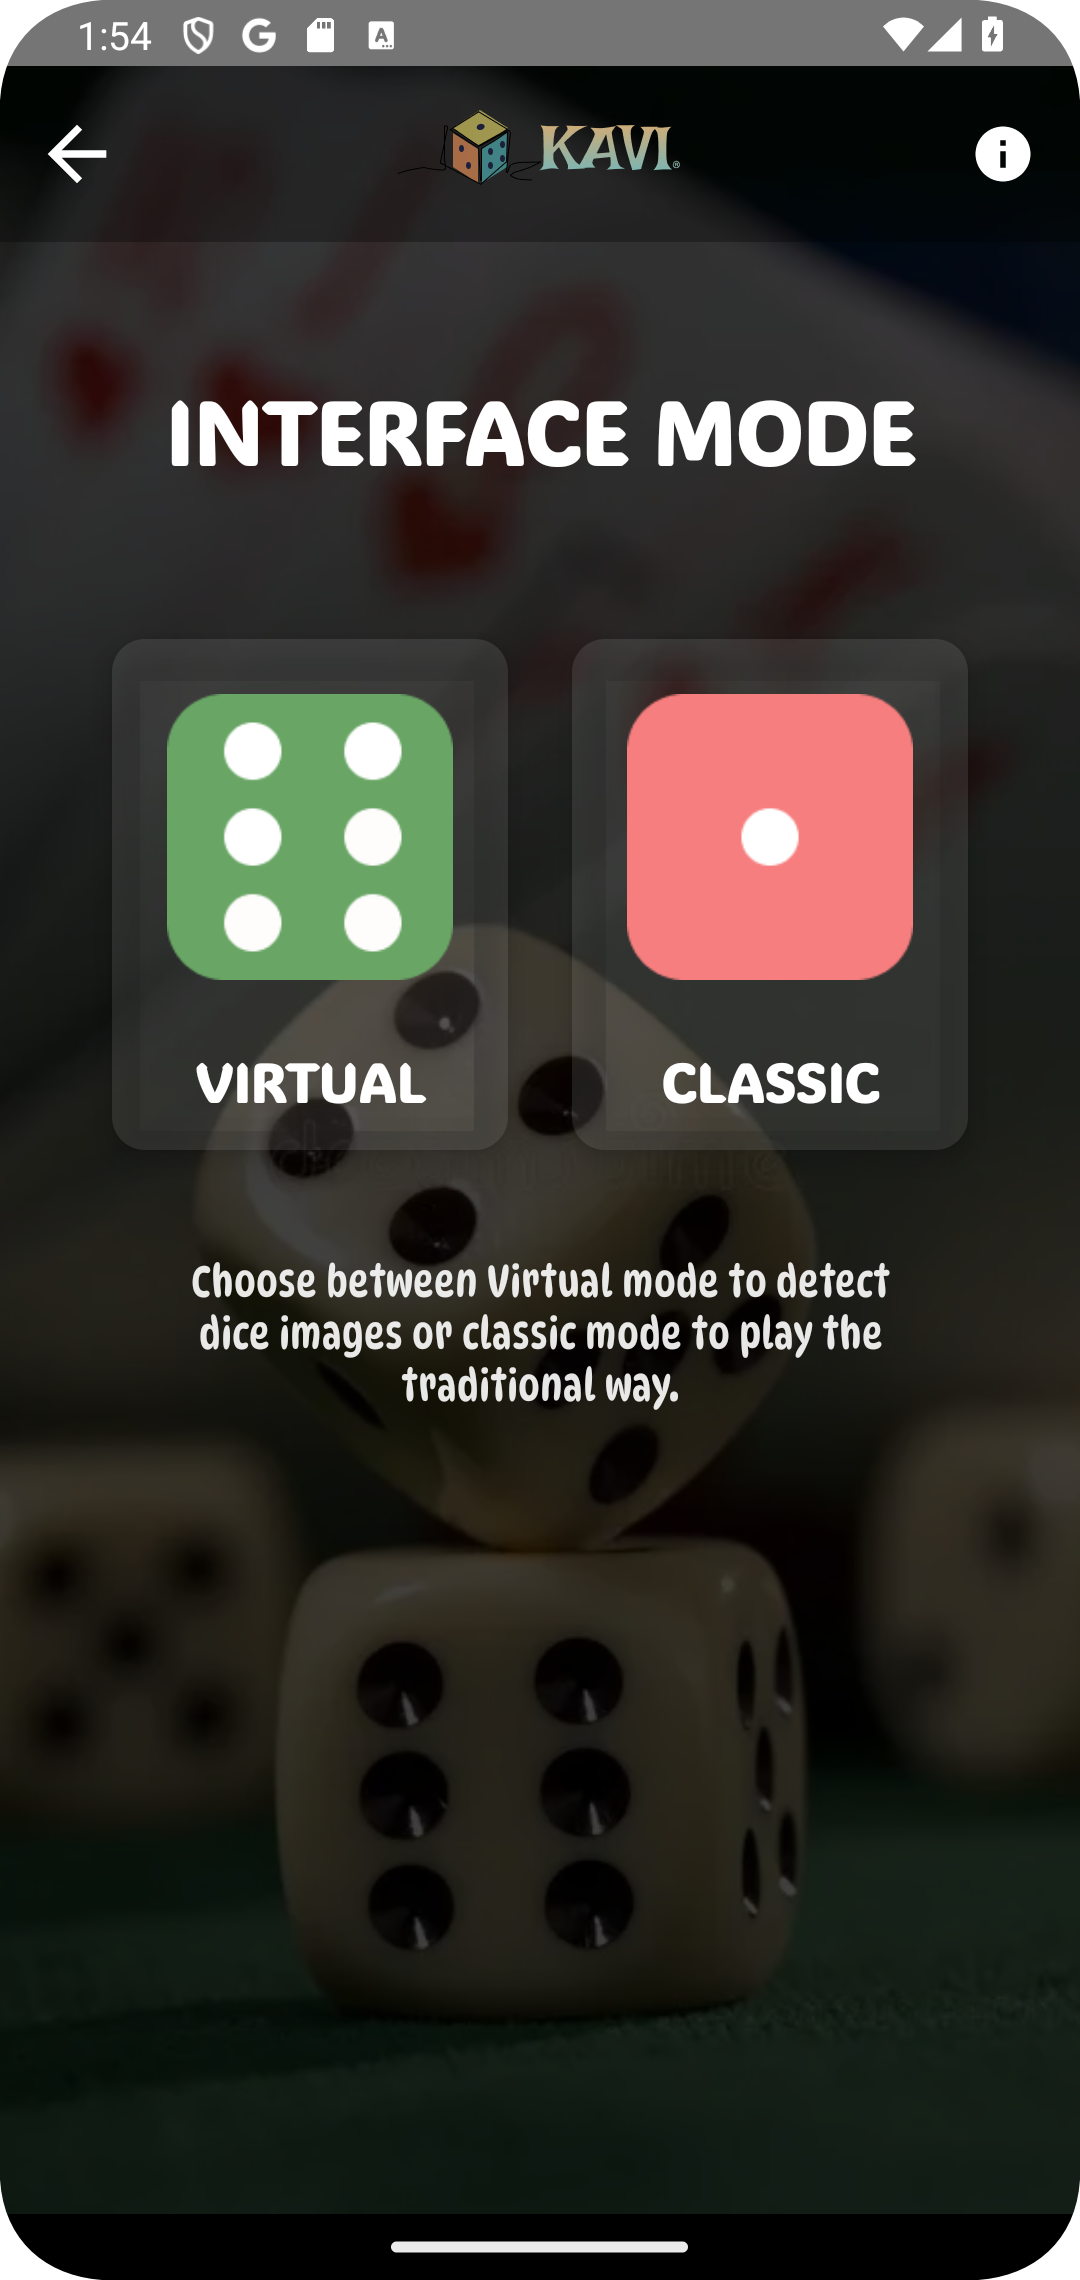
\includegraphics[width=\textwidth]{img/interface mode.png}
        \caption{The Start Screen}
        \label{fig:start_screen}
    \end{subfigure}
    \hfill
    \begin{subfigure}[b]{0.27\textwidth}
        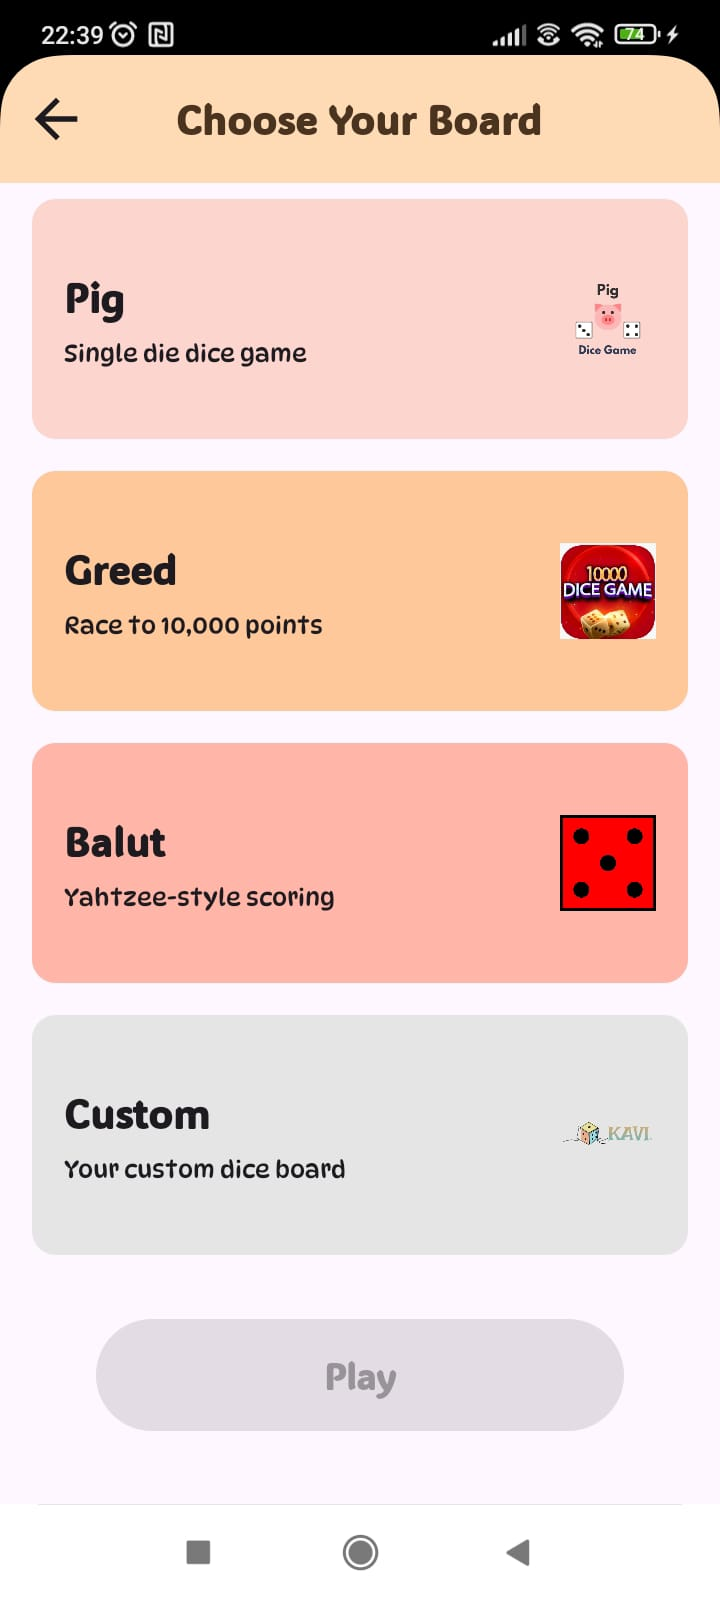
\includegraphics[width=\textwidth]{img/classic boards.jpg}
        \caption{Classic Mode}
        \label{fig:board_screen}
    \end{subfigure}
\caption{The Games main interfaces.}
\label{fig:interface_mode}
\end{figure}

\subsection{Classic Boards}

The application offers a diverse set of game boards, each designed for a distinct dice game experience. These games range from simple "press-your-luck" scenarios to more strategic challenges that require planning and risk management. The primary games offered are \textit{Pig}, \textit{Greed}, and \textit{Balut}. Additionally, the application includes a custom board where users can define their own game rules and scoring mechanisms, and also select the number of dice used in the game. The figure~\ref{fig:board_screen} shows the classic boards available in the application.

\begin{figure}[h]
    \centering
    \begin{subfigure}[b]{0.27\textwidth}
        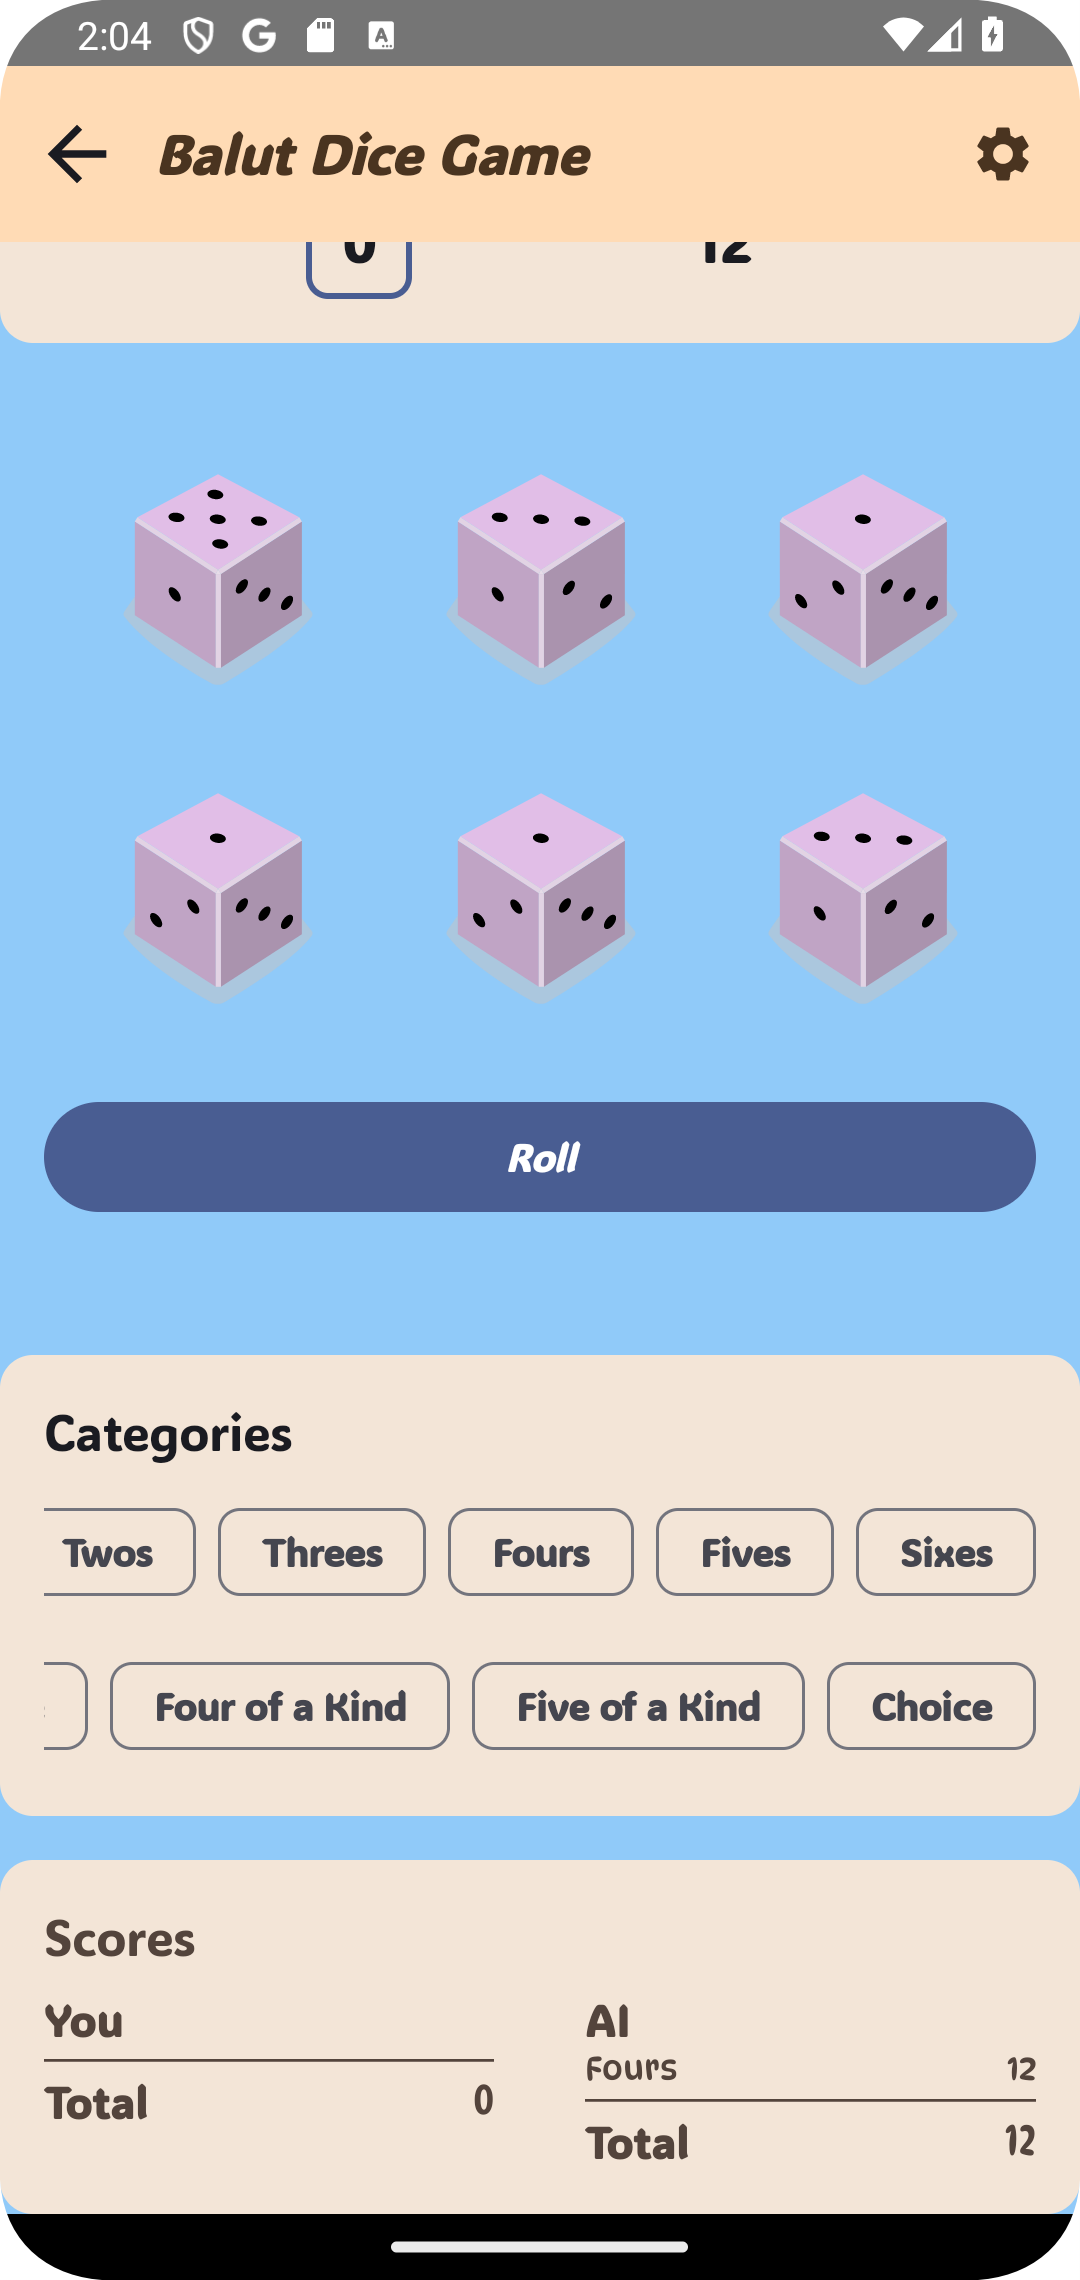
\includegraphics[width=\textwidth]{img/balut board.png}
        \caption{Balut Game Board}
    \end{subfigure}
    \hfill
    \begin{subfigure}[b]{0.27\textwidth}
        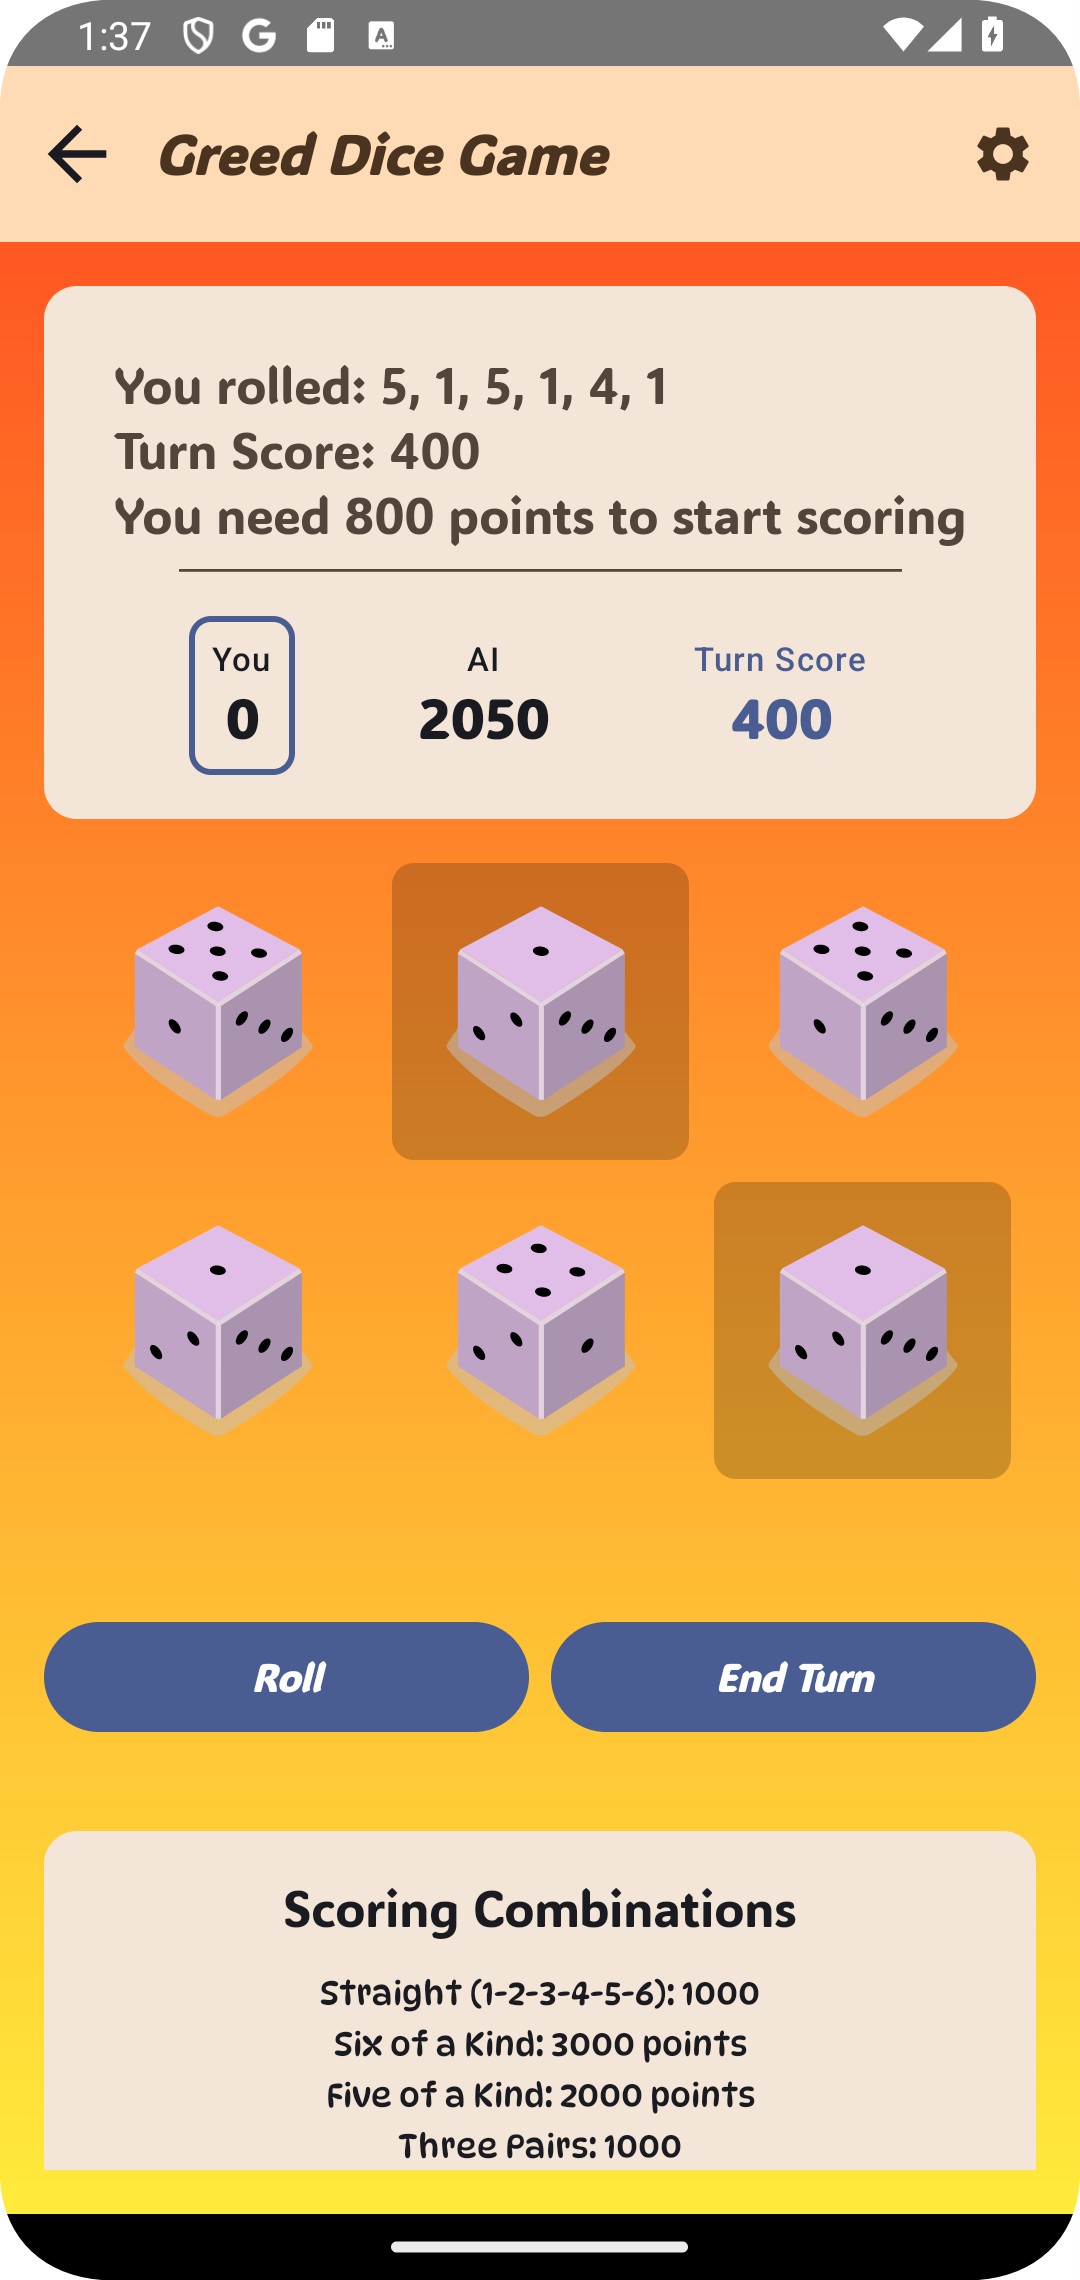
\includegraphics[width=\textwidth]{img/greed board.png}
        \caption{Greed Game Board}
    \end{subfigure}
    \hfill
    \begin{subfigure}[b]{0.27\textwidth}
        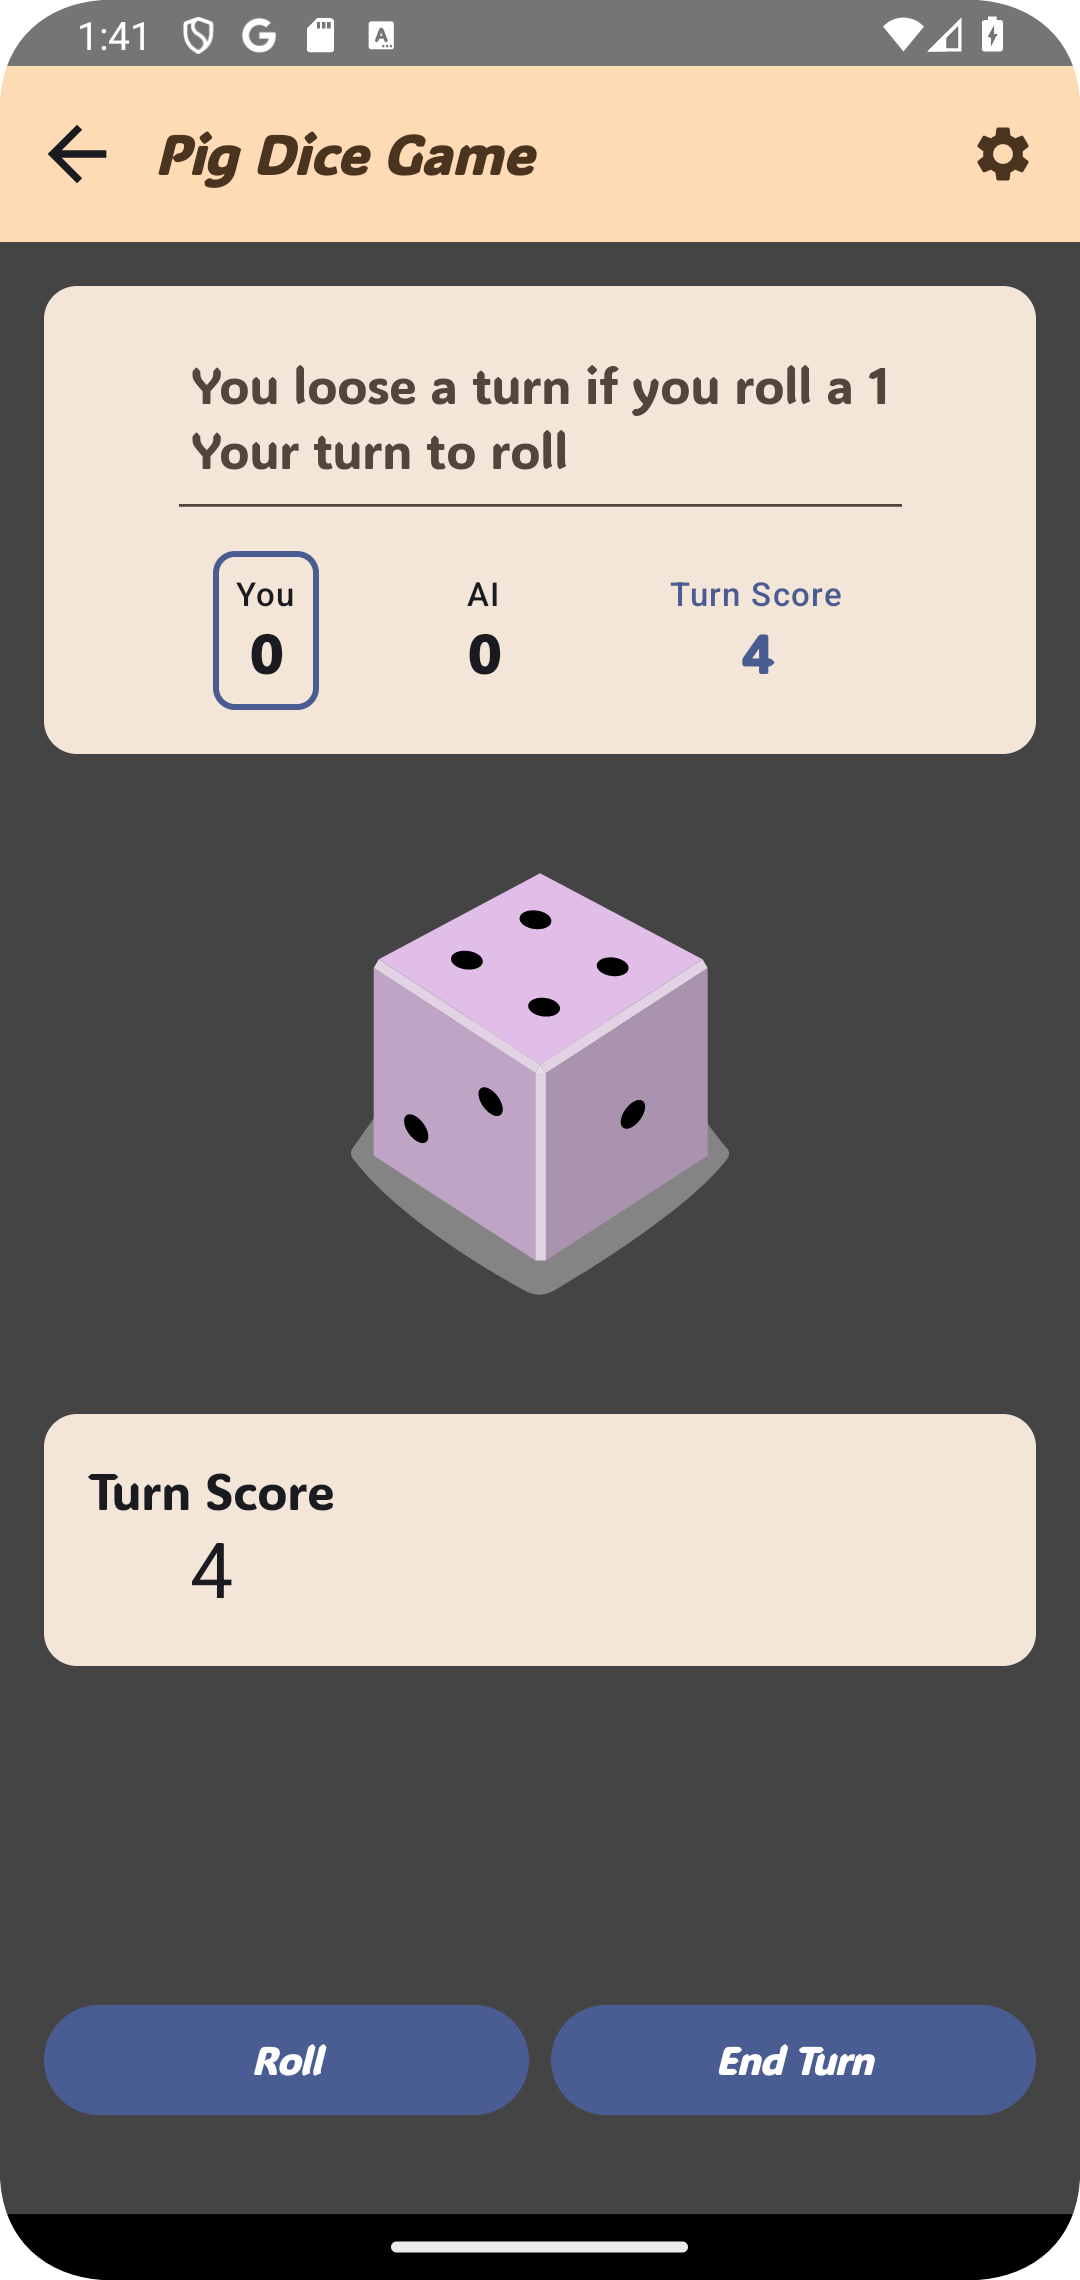
\includegraphics[width=\textwidth]{img/pig board.png}
        \caption{Pig Game Board}
    \end{subfigure}
    \caption{Game Boards in the Application}
\end{figure}

\subsection{Game Objectives}

\subsubsection{Pig: The Risk of the Roll}

Pig is a simple, engaging game of chance and risk. The goal is to be the first player to reach a total of 100 points. During each turn, players roll a single die, accumulating points with each roll. The key aspect of Pig is the ability to "bank" the points you have accumulated in that turn, however, the risk is that if you roll a 1, you lose all the points accumulated during that turn. The challenge lies in choosing when to press your luck for more points and when to play it safe to avoid losing those points.

\subsubsection{Greed: Navigating Scoring Combinations}

Greed is a more complex game that rewards strategic decision-making and risk-taking. Each turn begins with the roll of six dice. After the roll, players get to select which dice they want to keep to accumulate points, based on scoring combinations like straights, sets (e.g., three-of-a-kind, four-of-a-kind), and single 1s and 5s. These combinations vary in their scoring values, meaning that a key aspect of the game is knowing which combinations you should aim for. Unlike Pig, in Greed, players must accumulate at least 800 points in a turn to start banking them. The winner is the first player to reach a total of 10,000 points.

\subsubsection{Balut: Strategic Category Management}

Balut is a game of strategy, similar to Yahtzee. Players have up to three rolls per turn using five dice. The core of Balut is strategically filling the scoring categories, such as sets, straights, full houses, and more. Each category can be used only once, so planning and smart selection of which dice to hold is critical. After all categories are filled, the player with the highest total score wins.

\subsection{Game Controls: Interacting with the Game}

The application provides a user-friendly interface with intuitive controls, allowing players to easily interact with each game and manage their scores. This section talks about the various controls and how they function across different game modes.

\subsubsection{Basic Game Controls (Roll, End Turn)}

The primary way players interact with the games is through the roll button. In games like \textit{Pig} and \textit{Greed}, this button (shown in Figure \ref{fig:control1}) also serves as an "End Turn" button. In these games, tapping the button rolls the dice and also ends the turn after a score is obtained.

\begin{figure}[ht!]
    \centering
    
\includegraphics[width=0.6\textwidth]{img/control1.jpg}
    \caption{Roll and End Turn Button}
    \label{fig:control1}
\end{figure}

\subsubsection{Player Management and Custom Game Setup}

In the custom game board, it is also possible to add players and edit their names (as shown in Figure \ref{fig:control2}). This function can be accessed by tapping a button which allows the player to add and remove player, as well as edit their names. This allows users to set up a new game of their liking.

\begin{figure}[ht!]
    \centering
    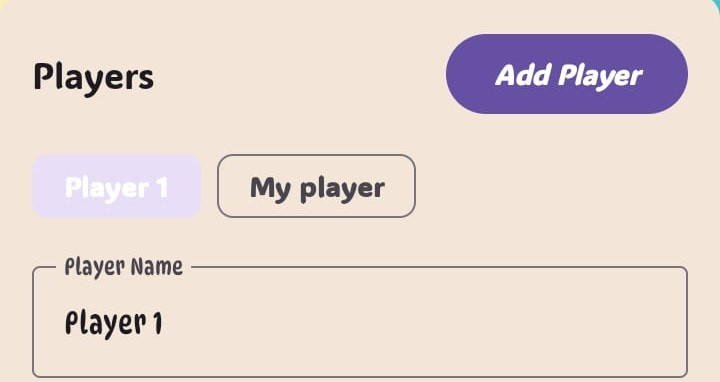
\includegraphics[width=0.6\textwidth]{img/control2.jpg}
    \caption{Player Management and Editing}
    \label{fig:control2}
\end{figure}

\subsubsection{Balut-Specific Controls (Category Selection)}

\textit{Balut} introduces the unique feature of category selection. After rolling the dice, a player can select a category in which to score, shown in Figure \ref{fig:control3}. This allows for a more strategic game, where each category can only be used once.

\begin{figure}[ht!]
    \centering
    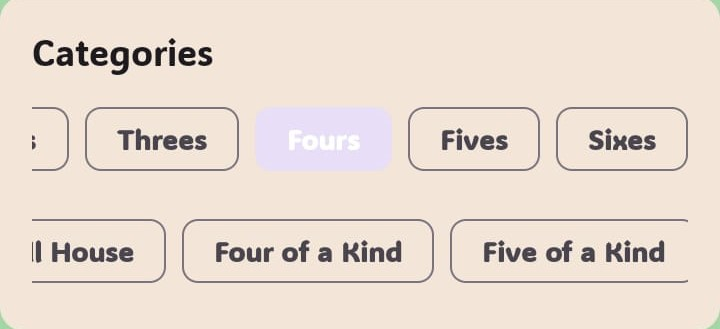
\includegraphics[width=0.6\textwidth]{img/control3.jpg}
    \caption{Balut Category Selection}
    \label{fig:control3}
\end{figure}

\subsubsection{Holding Dice}

In both \textit{Greed} and \textit{Balut}, players can strategically select dice to hold for the next roll. As seen in Figure \ref{fig:control4}, this is done by tapping on the individual dice on the screen. The selected dice will be saved, and can be rolled again in the subsequent roll.

\begin{figure}[ht!]
    \centering
    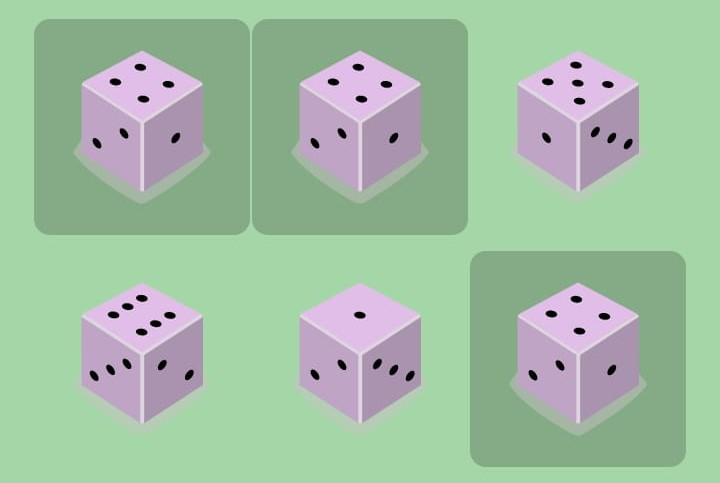
\includegraphics[width=0.6\textwidth]{img/control4.jpg}
    \caption{Selecting Dice to Hold}
     \label{fig:control4}
\end{figure}

\subsubsection{Balut Score Function}

After a category has been selected in \textit{Balut}, the game also provides an additional button which can be tapped to calculate the score and end the turn. As seen in figure \ref{fig:control5}.

\begin{figure}[ht!]
    \centering
    
\includegraphics[width=0.6\textwidth]{img/control5.jpg}
    \caption{Balut Roll and Score Button}
    \label{fig:control5}
\end{figure}

\subsubsection{Custom Board Settings}

The custom board allows players to set the number of dice that will be used for that specific game. In addition, the board name can also be set, as seen in Figure \ref{fig:control6}. This level of customization gives the users control over how the games are played.

\begin{figure}[ht!]
    \centering
    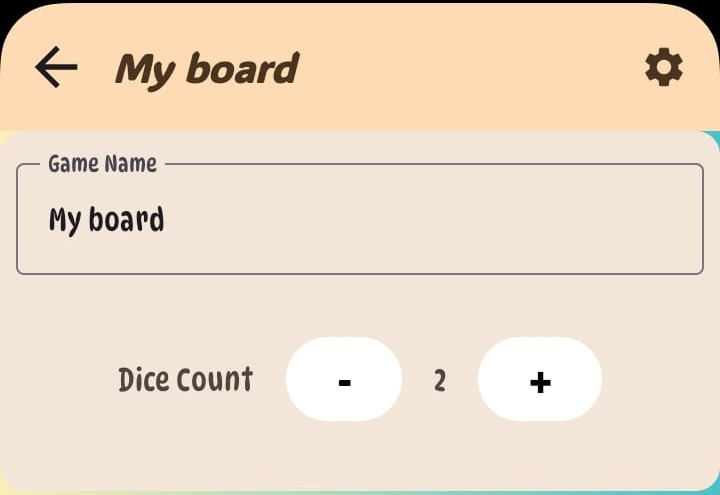
\includegraphics[width=0.6\textwidth]{img/control6.jpg}
    \caption{Custom Board Settings}
    \label{fig:control6}
\end{figure}

\subsubsection{Score Modifiers and Reset}

Figure \ref{fig:control7} shows the score modifiers, which enable users to manually adjust their scores. This feature can also be used to keep track of score in other types of games that might not be covered by this application, or in the custom mode. The feature also contains a reset score button that will reset the score of the game to 0. This can be used to easily restart any game or any other custom use. Additionally, this interface also contains the functionality of adding a note that will be saved as part of the game, which can be used to keep track of important information of the current game.

\begin{figure}[ht!]
    \centering
    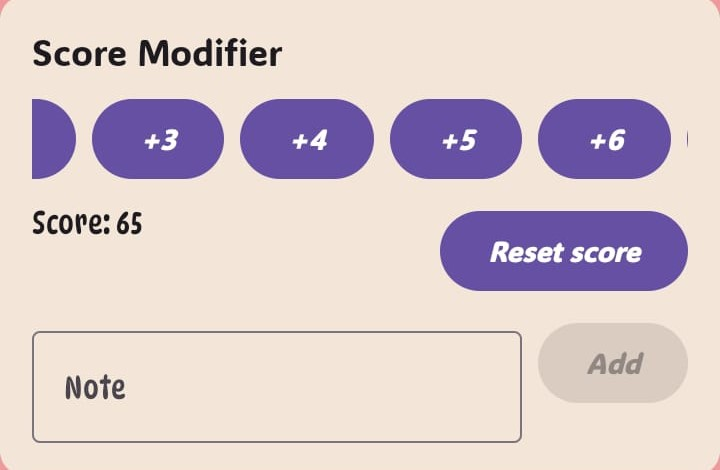
\includegraphics[width=0.6\textwidth]{img/control7.jpg}
    \caption{Score Modifiers and Reset}
     \label{fig:control7}
\end{figure}

\subsection{Instruction}

The instructions screen provides users with detailed guidance on how to play the game. It includes rules, tips, and strategies to enhance the gaming experience. The instructions screen is illustrated in Figure~\ref{fig:instructions_screen}.

\subsection{Settings}
The settings screen, on the other hand, allows users to customize their gaming experience, such as enabling vibration, the shake-to-roll function, and board color customization. The settings screen is shown in Figure~\ref{fig:settings_screen}.

\begin{figure}[h]
    \centering
    \begin{subfigure}[b]{0.27\textwidth}
        \centering
        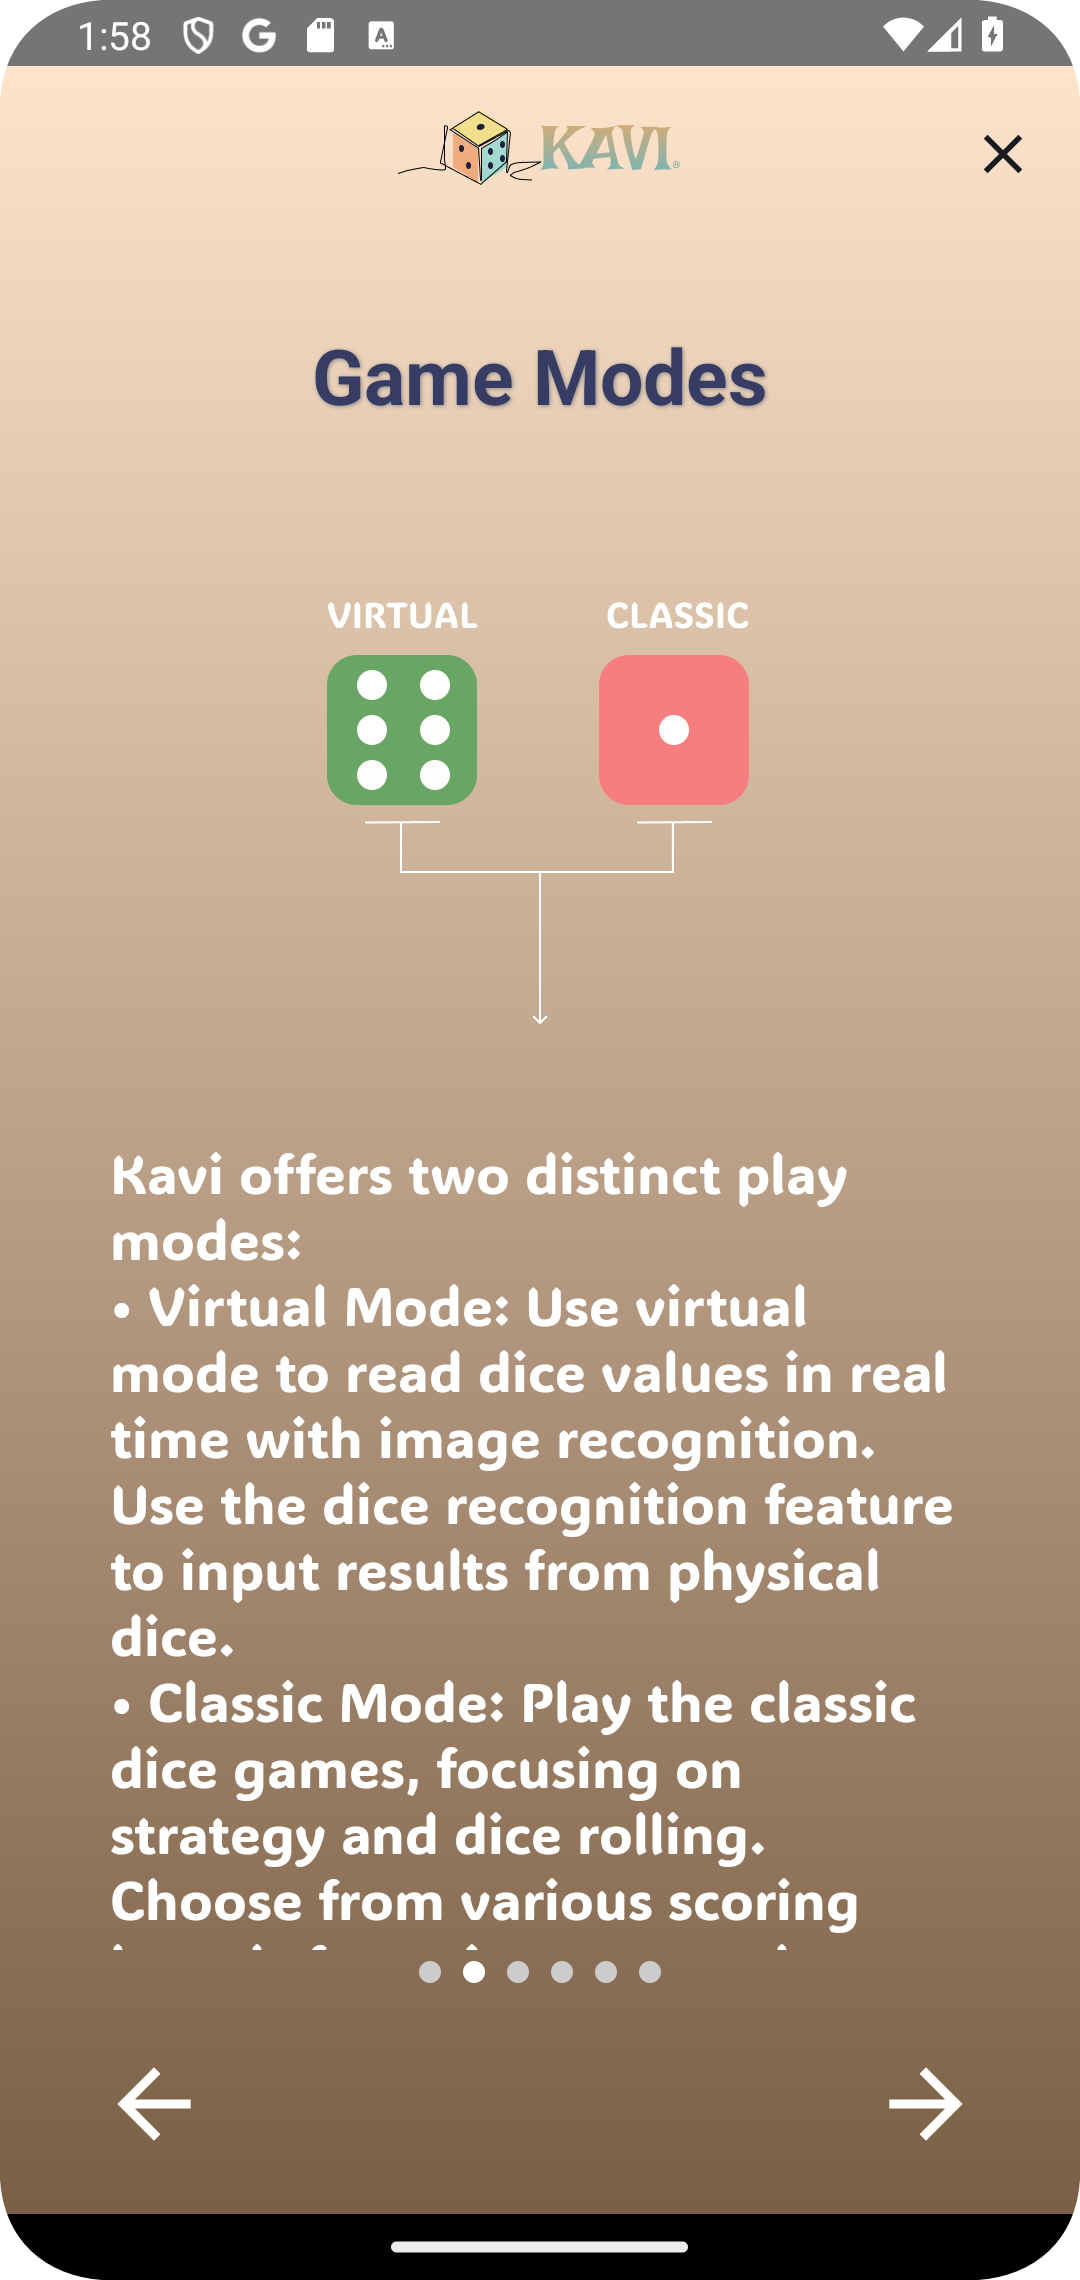
\includegraphics[width=\textwidth]{img/instructions screen.png}
        \caption{Instructions Screen}
        \label{fig:instructions_screen}
    \end{subfigure}
    \hspace{.5em}
    \begin{subfigure}[b]{0.27\textwidth}
        \centering
        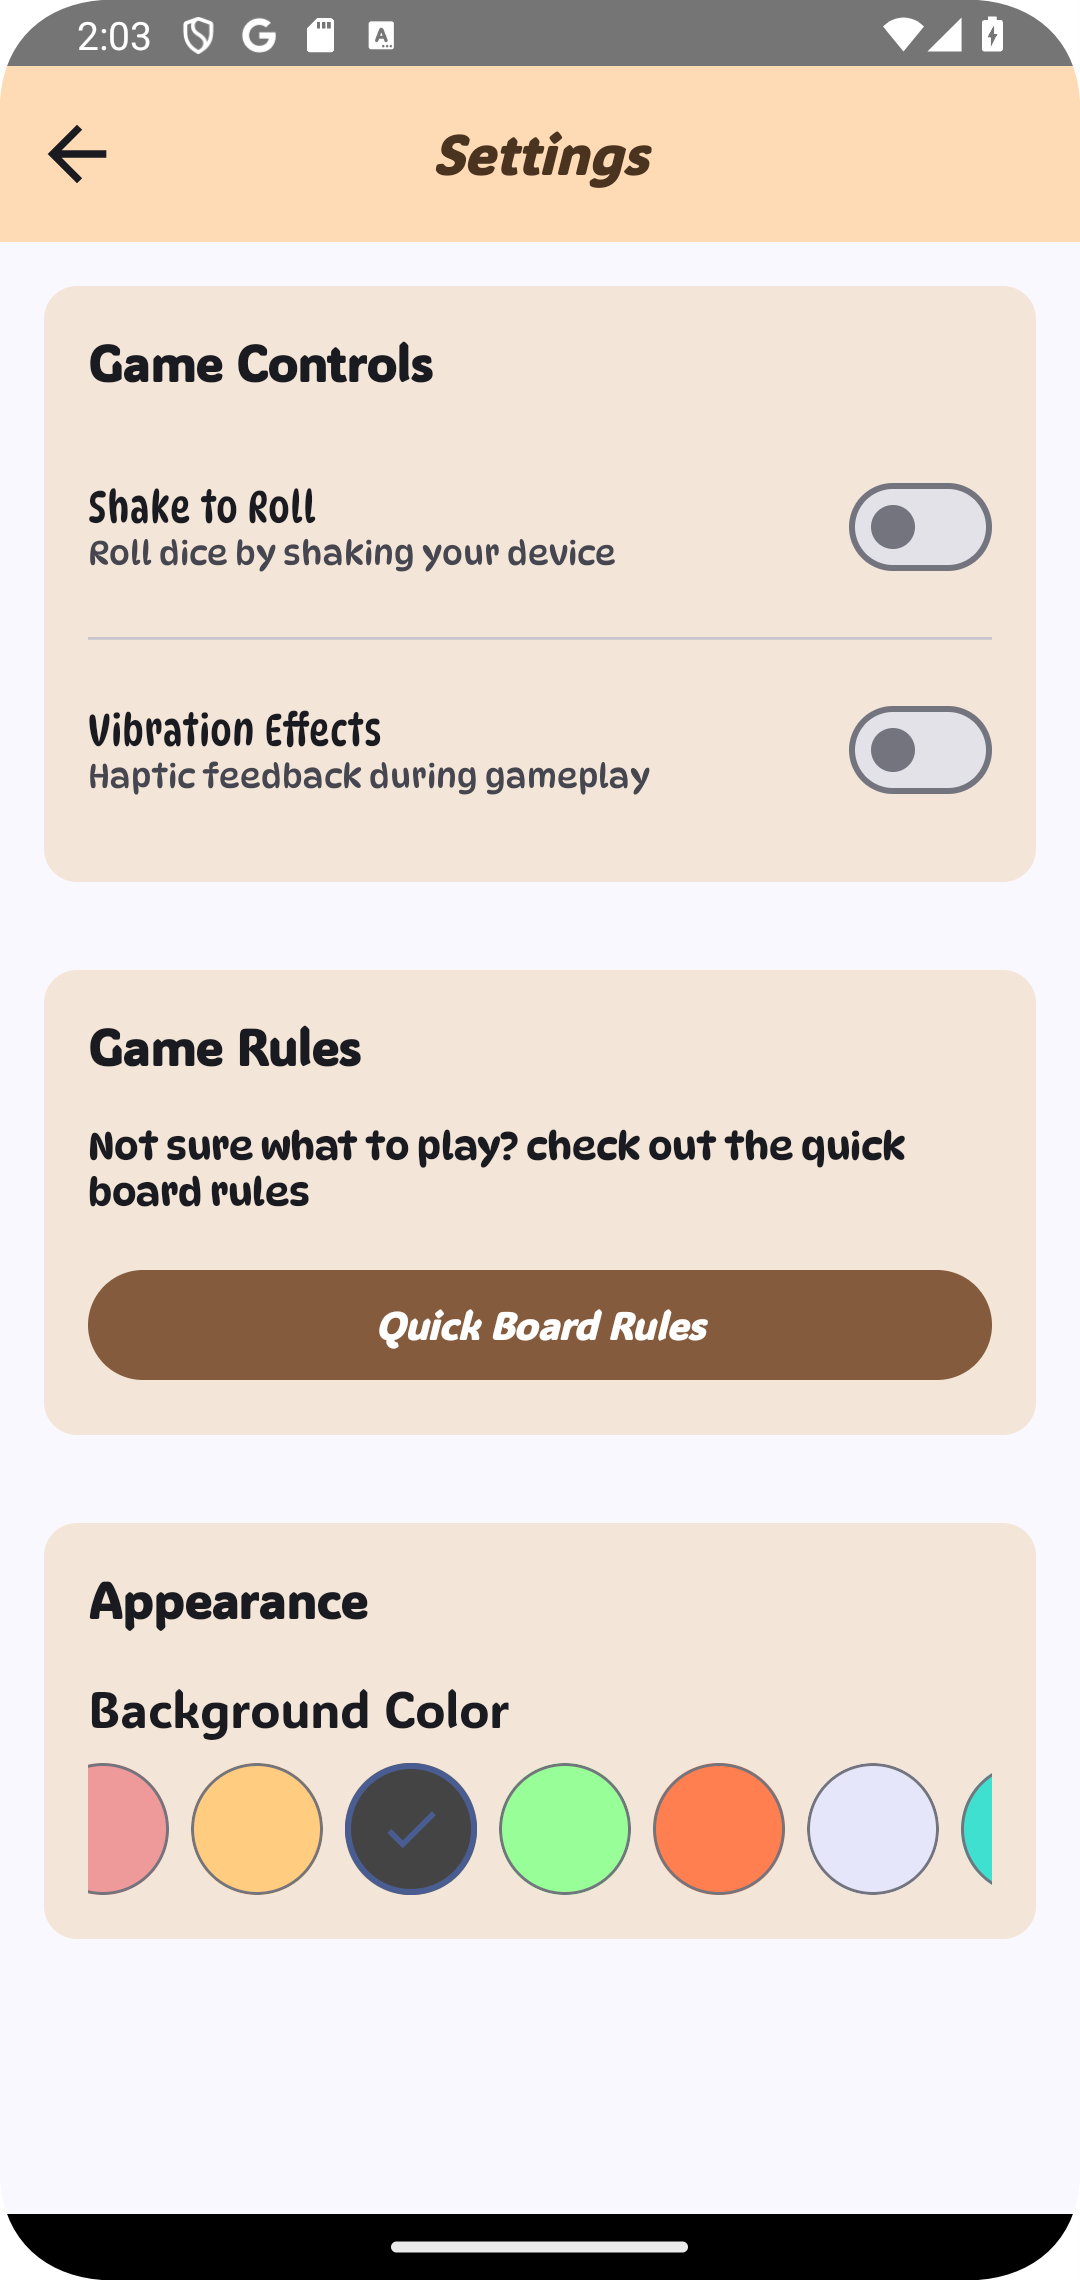
\includegraphics[width=\textwidth]{img/settings screen.png}
        \caption{Settings Screen}
        \label{fig:settings_screen}
    \end{subfigure}
    \caption{Instructions and Settings.}
\end{figure}

\subsection{Statistics}

The statistics screen offers users comprehensive insights into their gameplay performance. It displays a variety of data, including win records, average scores, and other pertinent metrics. The figure~\ref{fig:statistics_screen} illustrates the statistics screen, where users can view their achievements, such as "High Roller," "Lightning Fast," and "Greed Guru." Additionally, users can assess their risk-taking tendencies, current winning streaks, comebacks, and close games. The screen also features time analytics, allowing users to track their fastest games, total playtime, and time spent on individual games, providing a detailed overview of their gaming habits.
\begin{figure}[h]
    \centering
    \begin{subfigure}[b]{0.27\textwidth}
        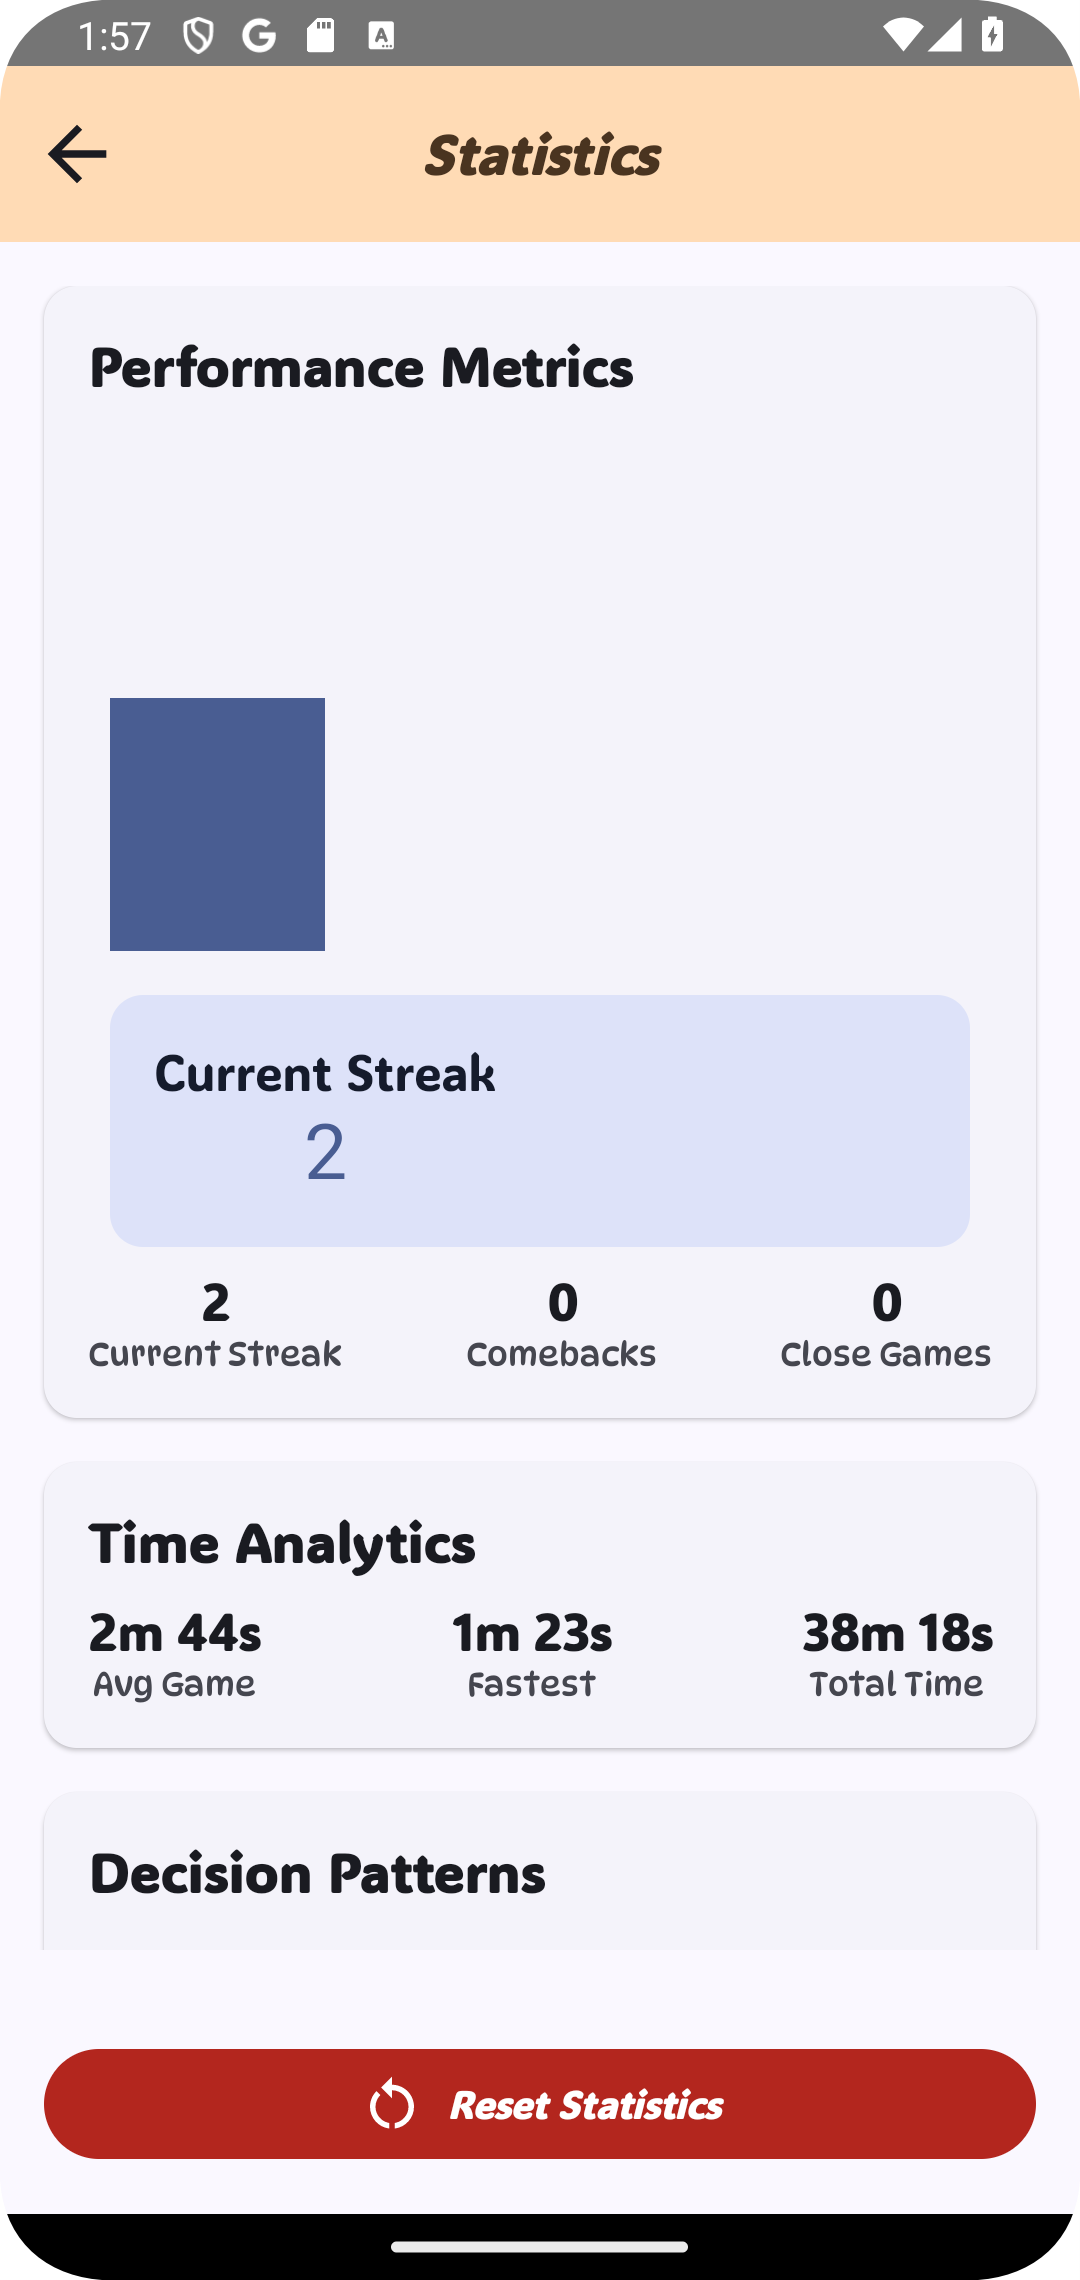
\includegraphics[width=\textwidth]{img/statistics screen.png}
        \caption{Performance Metrics}
    \end{subfigure}
    \hfill
    \begin{subfigure}[b]{0.27\textwidth}
        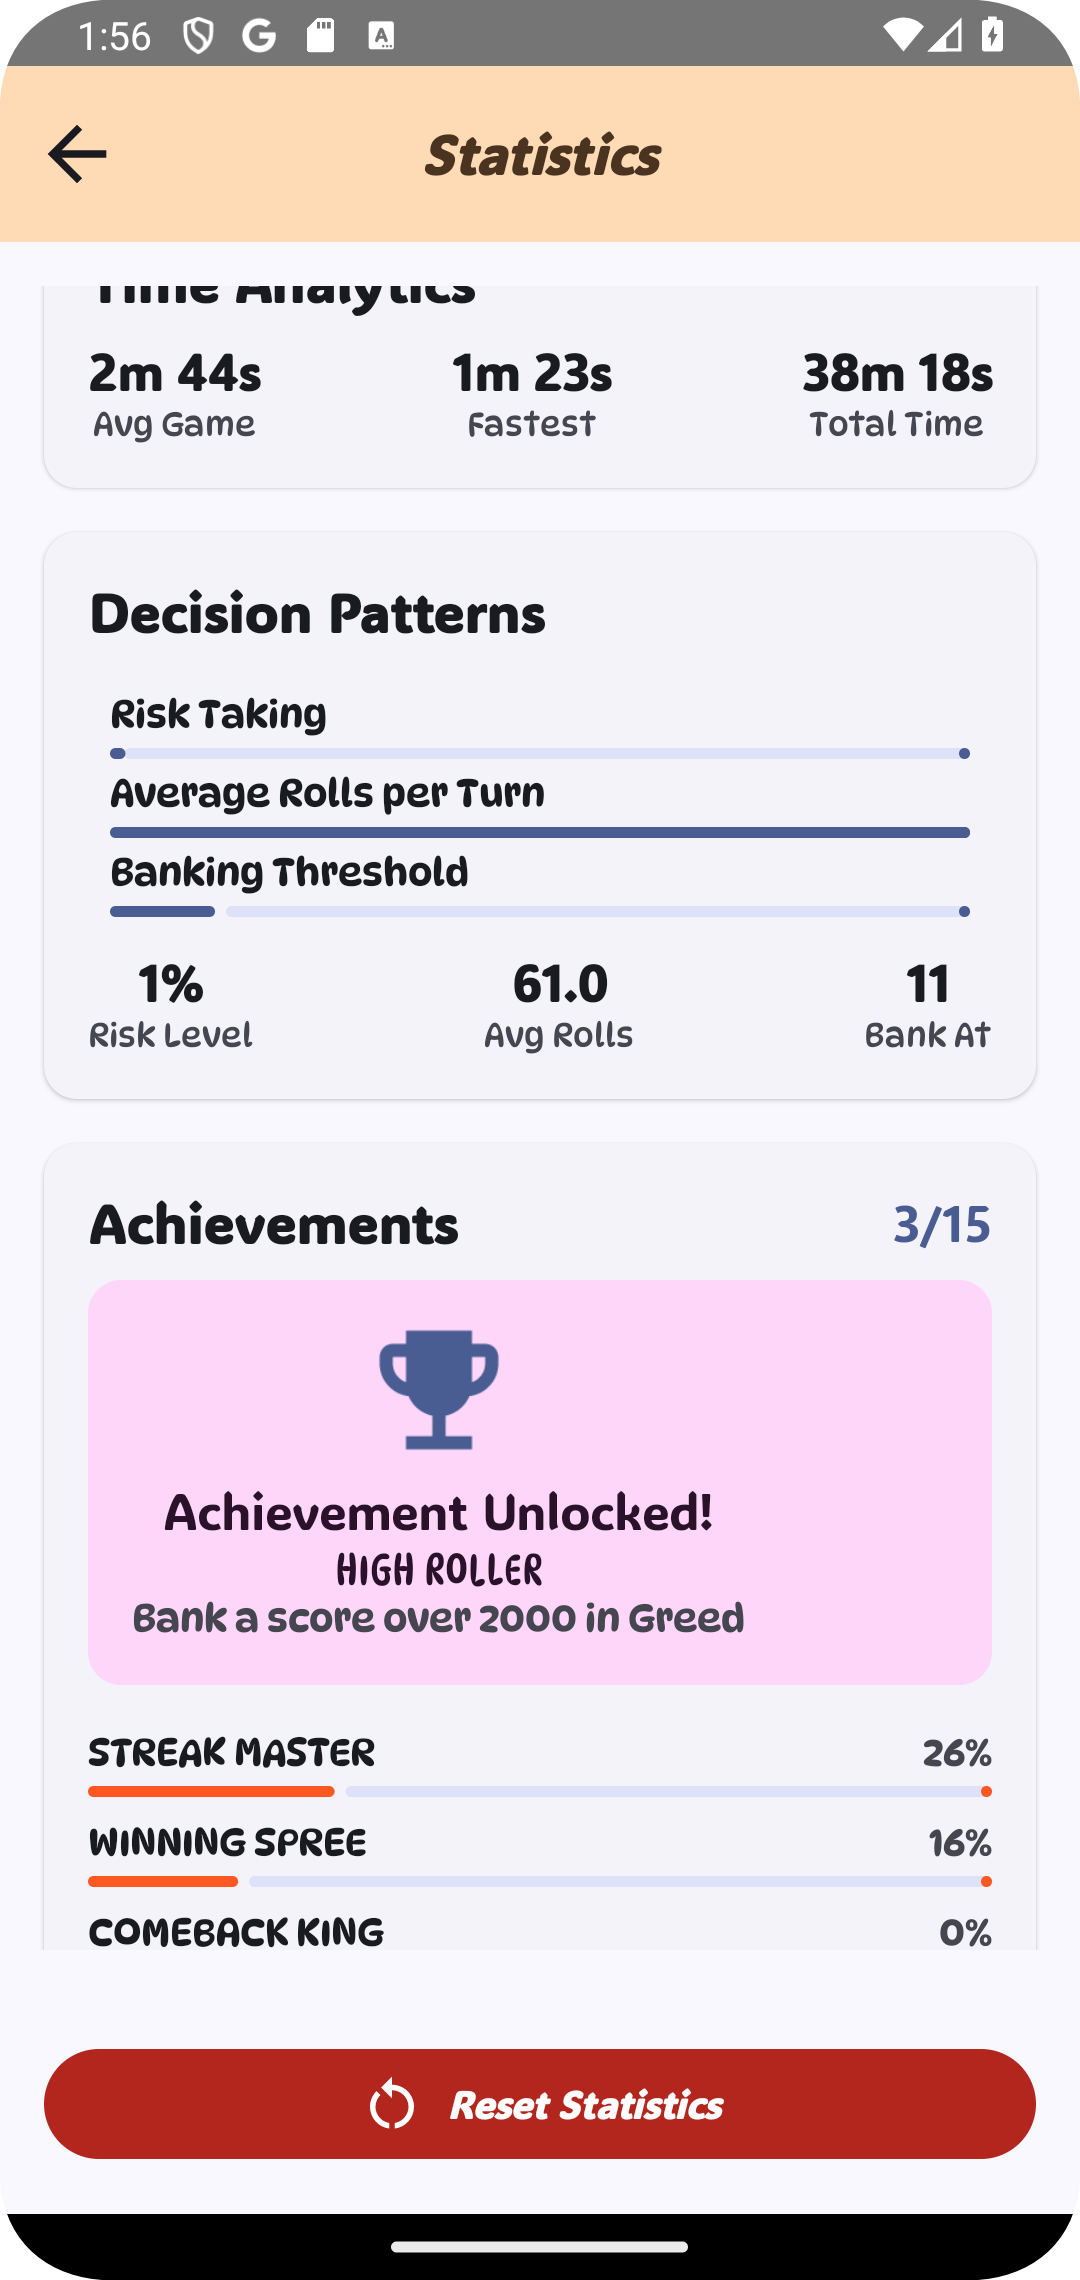
\includegraphics[width=\textwidth]{img/statistics screen3.png}
        \caption{Decision Patterns}
    \end{subfigure}
    \hfill
    \begin{subfigure}[b]{0.27\textwidth}
        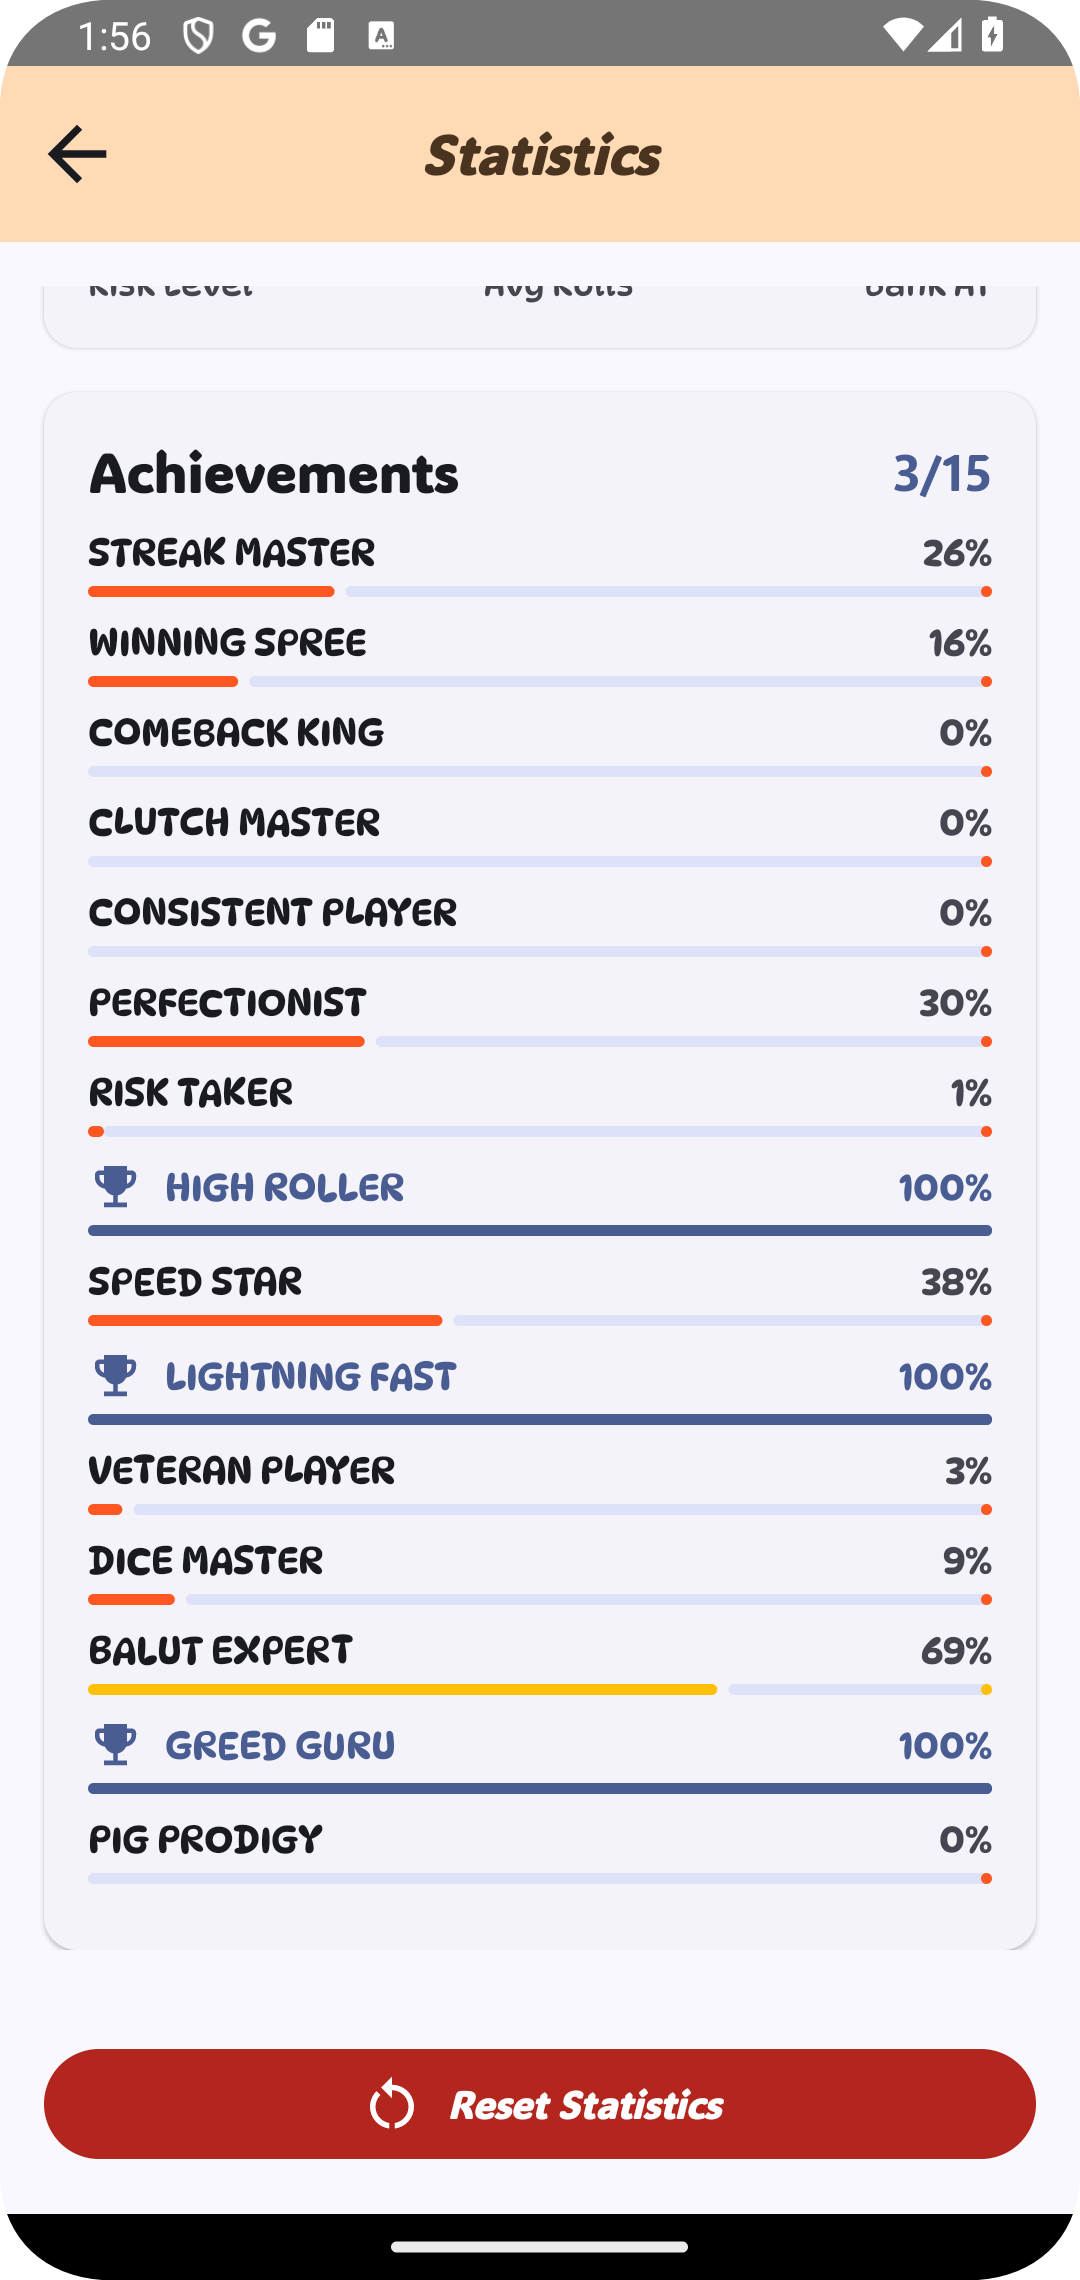
\includegraphics[width=\textwidth]{img/statistics screen2.png}
        \caption{Unlocking Achievements}
    \end{subfigure}
    \caption{Statistics Screen}
    \label{fig:statistics_screen}
\end{figure}

\section{System Administration}

The administration of the application involves several key tasks to ensure its reliability, performance, and security. These responsibilities are primarily carried out by the developers of the application, and can range from day to day maintenance to handling the occasional unforeseen issues.

\subsection{Application Maintenance}

Regular maintenance of the application is essential to ensure it remains functional and up to date. This involves several tasks, including:

\begin{itemize}
    \item \textbf{Release Management:} New releases of the application are periodically deployed via GitHub as APK releases, which often require careful planning and testing to ensure compatibility and maintain a consistent user experience. This includes creating new release branches, building the APK, and updating the app with new changes, new features, or bug fixes.
    \item \textbf{Monitoring and Troubleshooting:} Developers are also responsible for monitoring the performance of the application. This may involve checking for crashes, logging error reports, identifying bugs or unexpected behavior, and making changes to solve the issues.
\end{itemize}

\subsection{Data Management}

Careful management of the application data is critical to ensure its proper functioning.  The developers are responsible for \textit{DataStore Management}, which involves taking periodic backups of application settings and user preferences stored with Android DataStore. The data is also cleaned periodically to ensure that the device is not using unnecessary storage. This is essential to maintain consistency and avoid potential data corruption or data loss.

\section{Security Issues}
\subsection{Introduction}
This section provides a detailed view on the various security issues that the application is vulnerable to, based on potential threats and exploitable areas in the application.

\subsection{Data Handling}

Application data, including DataStore backups, might be accessed through Android's backup services if a user's Google account is compromised. Specifically, an attacker might be able to get access to the application if a user's Google account has been \textit{phished}, or if there has been a \textit{data breach}, or if the account has been compromised in some other way.

A compromised Google account could allow an attacker to access backups stored in Google Drive, potentially revealing all user information stored in the application.

The application uses Android's KeyStore to encrypt the backup data, however, this is not a full solution and does not prevent unauthorized access \cite{bib:android_data_backup}.

\subsection{Communication and API}
Even when using HTTPS, attackers can intercept data during transmission to the RoboFlow API. An attacker on the same network as the user can set up a malicious server and redirect all API requests to it, thereby gaining access to the API traffic. The application enforces HTTPS for all API requests, but it does not use certificate pinning, which means it is vulnerable to \textit{man in the middle} attacks. This is something that should be considered for future versions of the application. A sophisticated attacker could potentially bypass the HTTPS certificate and redirect the traffic through a malicious server. \cite{bib:owasp_top_ten}

Even with rate-limiting, attackers can bypass limitations and create a denial of service attack, potentially making the app or the external API unusable. A bot could flood the application with API requests. The application uses rate-limiting using a `CoroutineScope` and a `MutableStateFlow` to limit how many times an API is called in a given time, this does reduce the risk of the application crashing, but it is not foolproof. It also has input validation to prevent \textit{API abuse}, but these are not foolproof solutions and might be bypassed by sophisticated attackers.

\subsection{Code Security}

Even when using code obfuscation, attackers can still reverse engineer the code to steal private information and private API keys, or understand the game logic. Code Obfuscation is the process of making the code more difficult to read and understand, by changing the variable names, and classes to make them unreadable.

An attacker can decompile the application to find API keys that are used to contact external resources, or understand the game logic to make a bot to cheat at the game.

The application uses code obfuscation through R8's obfuscation process, to hide the code logic, which is not a full solution, and can be bypassed by sophisticated attackers \cite{bib:android_obfuscation}.

\section{Security Considerations}

The application implements several security measures to protect user data and ensure system integrity. These measures are based on Android security best practices and are designed to comply with relevant data protection requirements.

\subsection{Data Protection}

\begin{itemize}
    \item \textbf{Encrypted Local Storage:} User settings and preferences, saved using DataStore, are stored using Android's EncryptedSharedPreferences, which provides encryption at rest using Android's KeyStore.
    \item \textbf{Privacy-Preserving Image Processing:} Images captured by the user are only processed within the app's scope and are not stored or transmitted outside of the device unless explicitly requested by the user through a sharing action. No personally identifiable information is extracted and saved from the image.
\end{itemize}

\subsection{System Security}

\begin{itemize}
    \item \textbf{Runtime Permission Management:} The application requests only the necessary permissions at runtime (e.g., camera access) and respects the user's choice to grant or deny them. The application uses Android's Permission API to handle the permissions.
    \item \textbf{Secure Communication Channels:} The communication with the RoboFlow API for image recognition is done over HTTPS, which uses TLS/SSL encryption to ensure confidentiality and integrity of the API requests.
     \item \textbf{Data Access Controls:} Only the application can access the DataStore data, and only the specific components of the application that require it can access its underlying data. This reduces the risk of potential data exposure to malicious application or rogue modules of this application.
\end{itemize}

\subsection{Future Enhancements}

The following security enhancements are considered for future development:

\begin{itemize}
    \item \textbf{User Authentication and Authorization:}  Implementing a secure user authentication mechanism (e.g., using Firebase Authentication) and role-based authorization to enhance data protection and prevent unauthorized access to sensitive features, such as statistics or training data.
    \item \textbf{Improved API Security:} Implementing API rate-limiting to prevent abuse and implementing stricter input validation for the RoboFlow API.
     \item \textbf{Regular Security Audits:} Implementing regular penetration testing to evaluate the security and performance of the system.
\end{itemize}

\section{Working scenarios}

In addition to the scenarios described in the user manual \ref{sec:user_manual}, this section provides a few practical examples of application usage.

\begin{figure}[h]
    \centering
    \begin{subfigure}[b]{0.27\textwidth}
        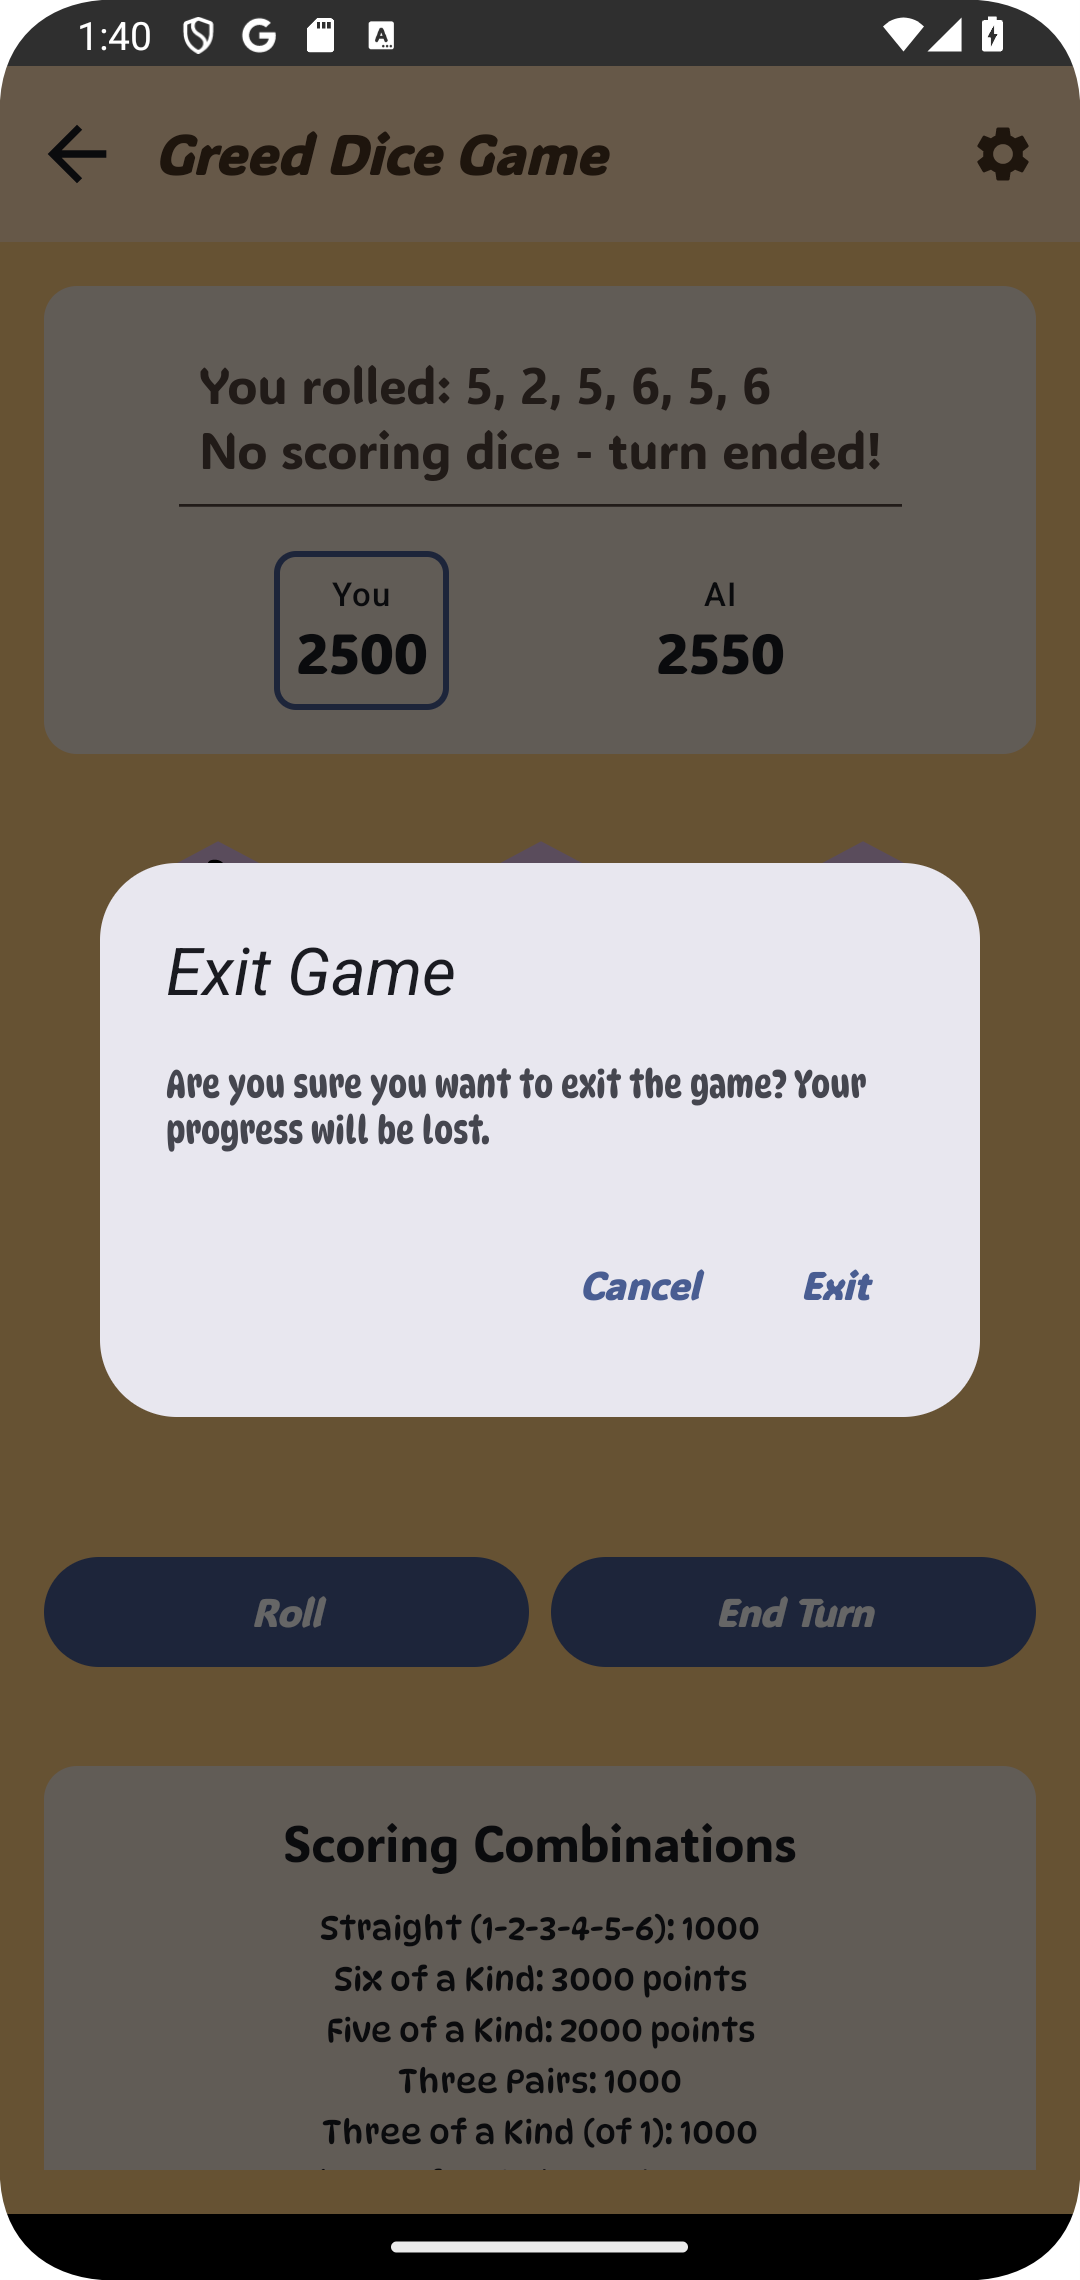
\includegraphics[width=\textwidth]{img/greed board2.png}
        \caption{Exiting a game of Greed}
    \end{subfigure}
    \hfill
    \begin{subfigure}[b]{0.27\textwidth}
        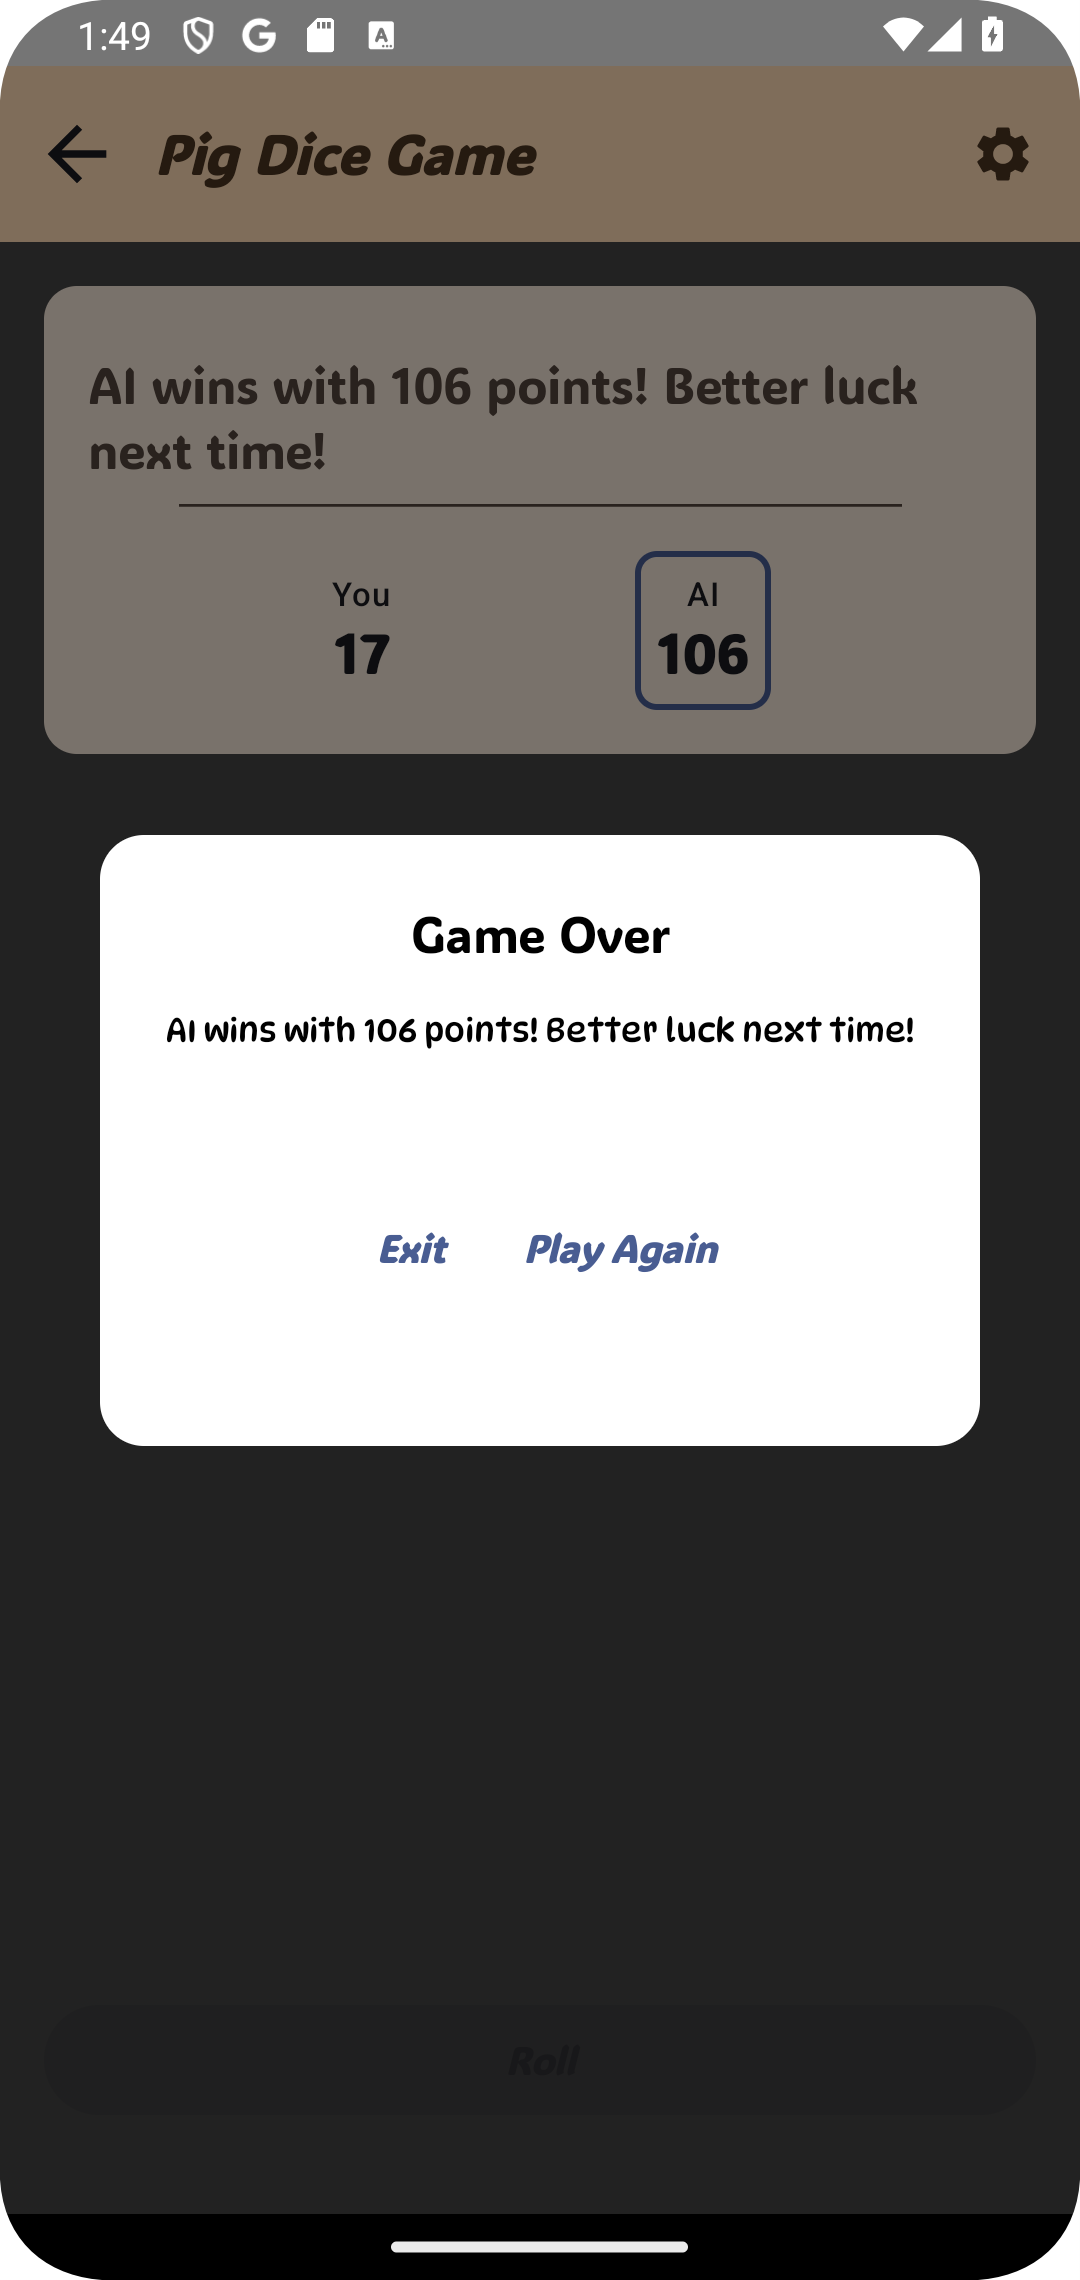
\includegraphics[width=\textwidth]{img/pig board2.png}
        \caption{Loosing a Game of Pig}
    \end{subfigure}
    \hfill
    \begin{subfigure}[b]{0.27\textwidth}
        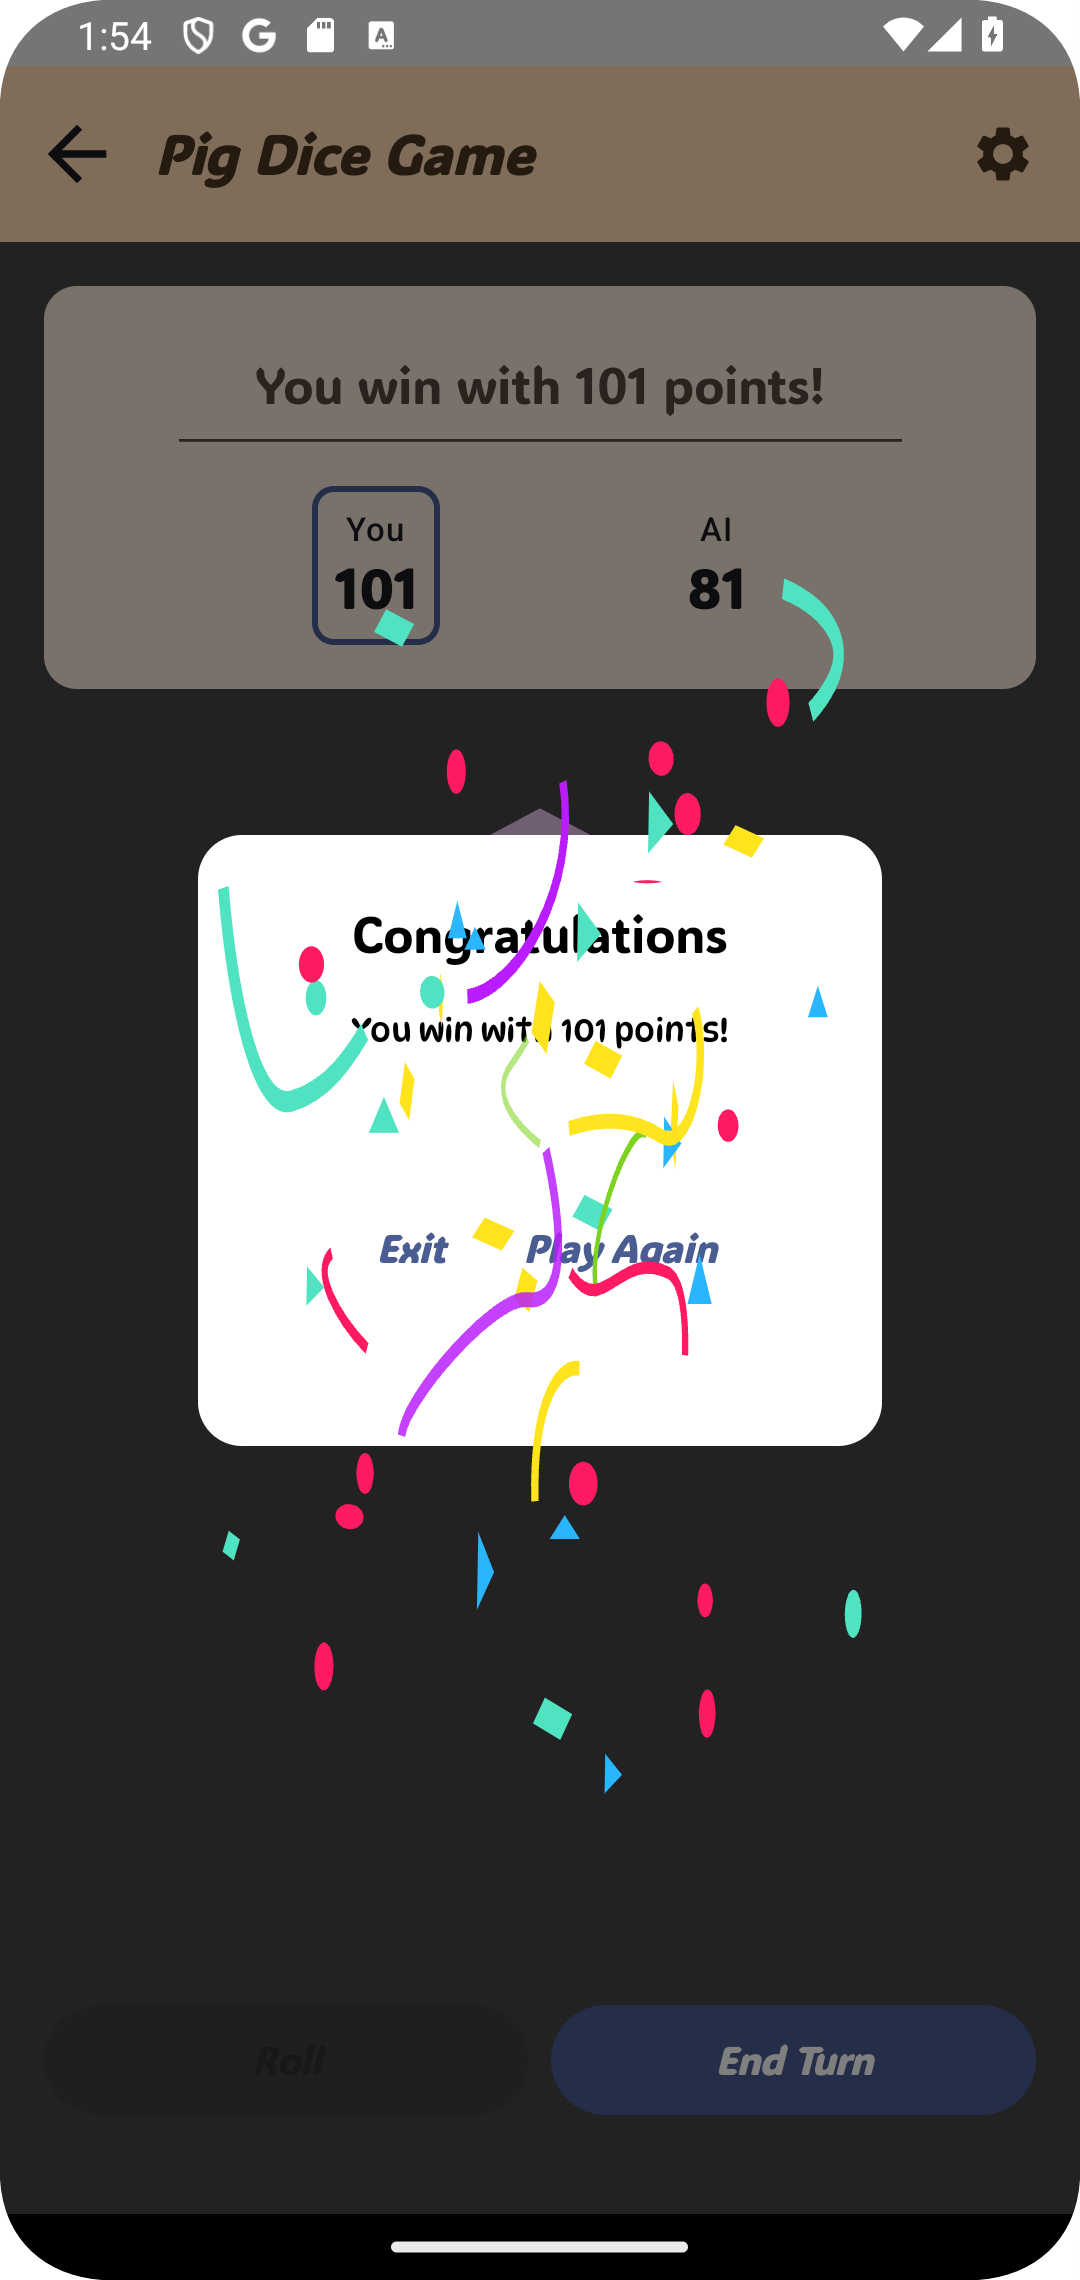
\includegraphics[width=\textwidth]{img/pig board3.png}
        \caption{Winning a Game of Pig}
    \end{subfigure}
    \caption{Board Features in the Application}
\end{figure}

\begin{figure}[ht!]
    \centering
    \begin{subfigure}[b]{0.27\textwidth}
        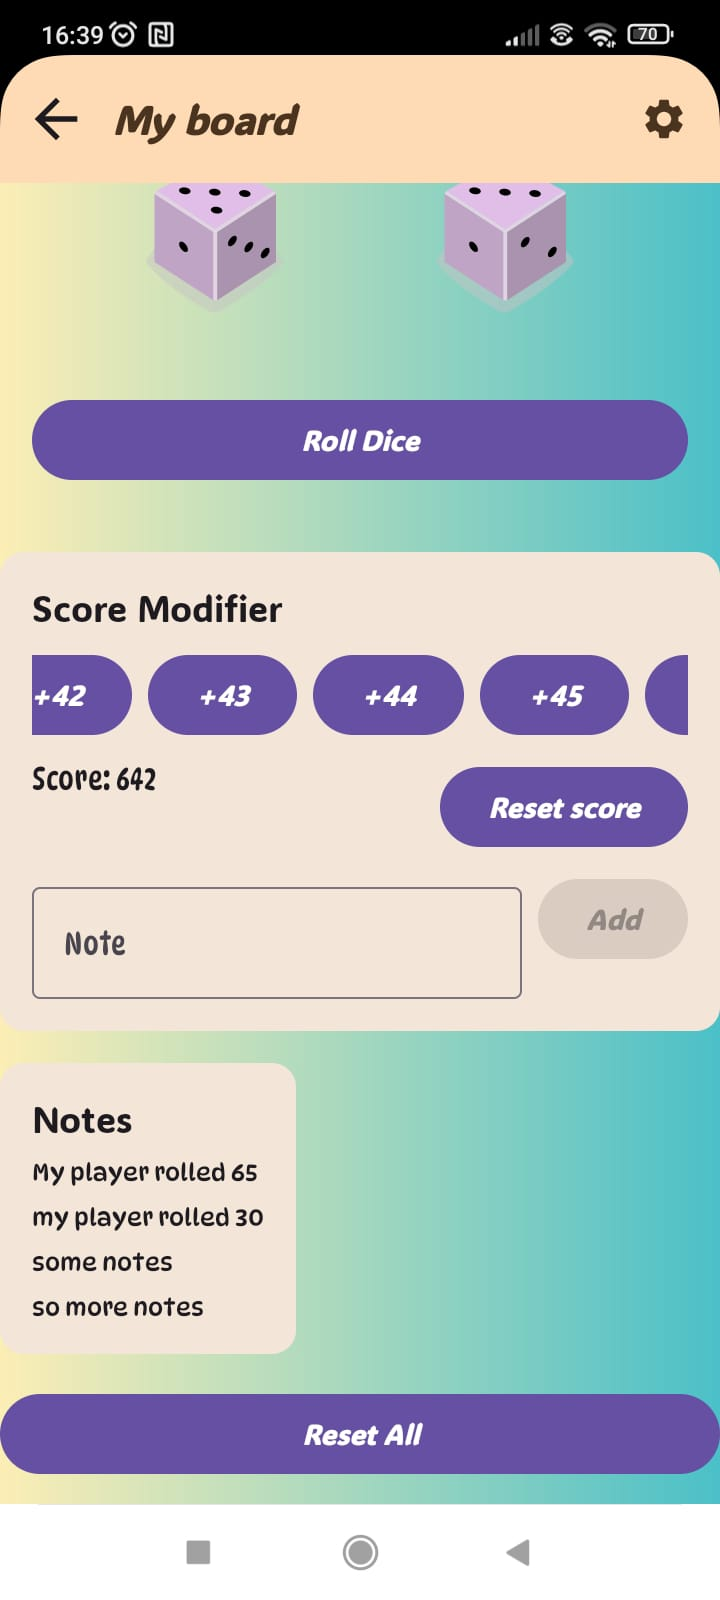
\includegraphics[width=\textwidth]{img/custom game.jpg}
        \caption{Custom Game Board}
    \end{subfigure}
    \hfill
    \begin{subfigure}[b]{0.27\textwidth}
        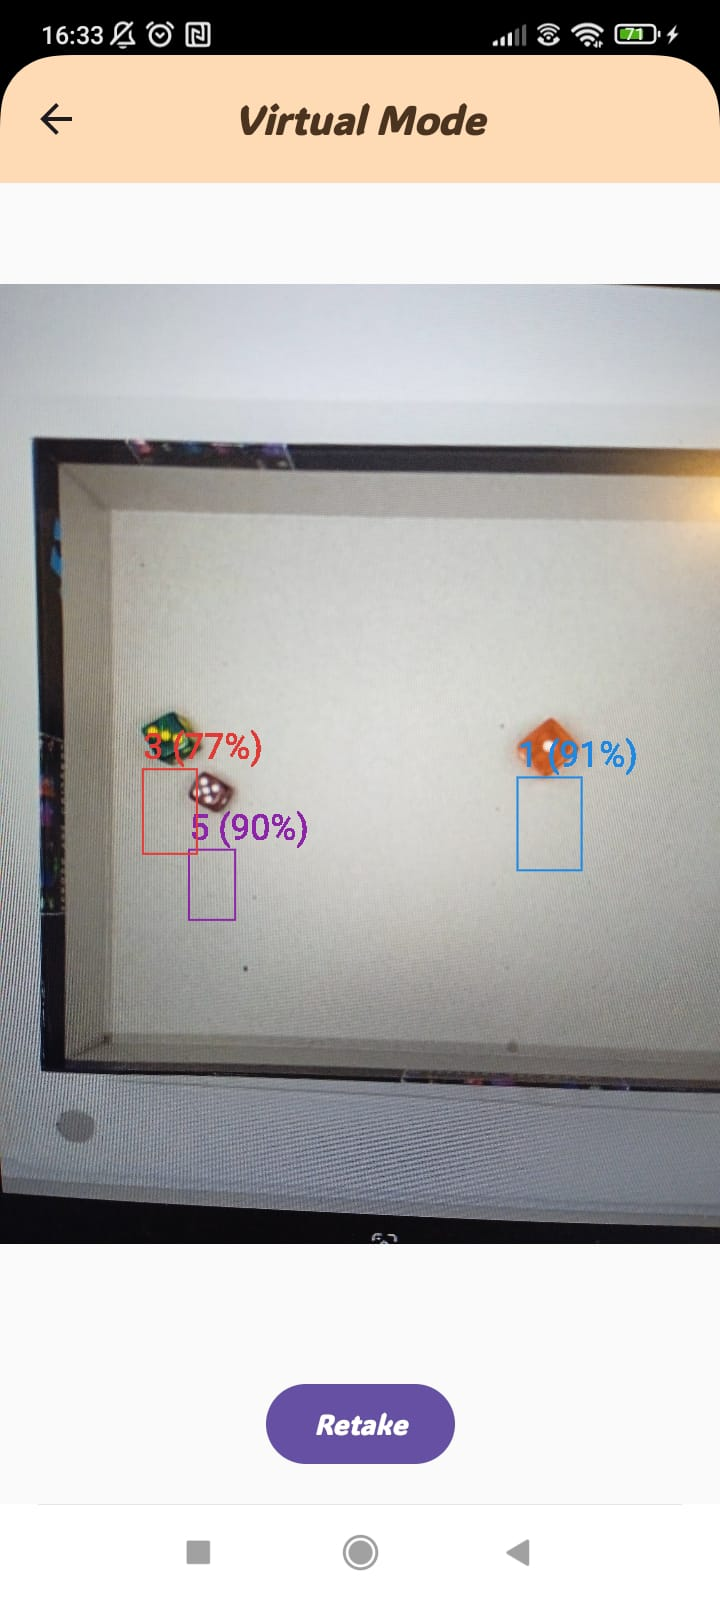
\includegraphics[width=\textwidth]{img/virtual screen2.jpg}
        \caption{Image Recognition Example}
    \end{subfigure}
    \hfill
    \begin{subfigure}[b]{0.27\textwidth}
        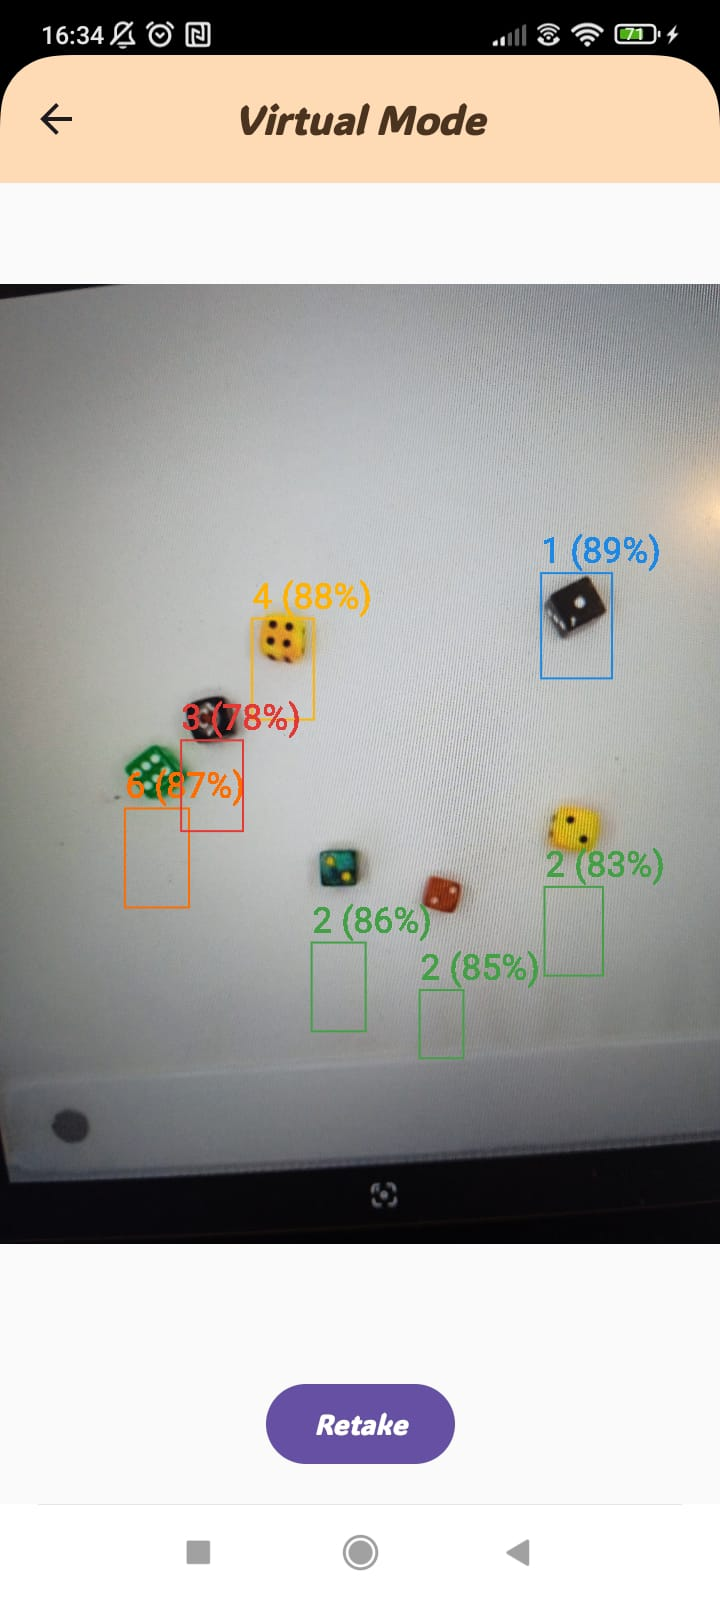
\includegraphics[width=\textwidth]{img/virtual screen.jpg}
        \caption{Image Recognition Example 2}
    \end{subfigure}
    \caption{Additional Features and Interactions}
\end{figure}